\documentclass[UTF8,12pt,a4paper]{ctexart}

\usepackage{amsmath,amssymb}
\usepackage{booktabs}
\usepackage{array}
\usepackage{geometry}
\usepackage{graphicx}
\usepackage[hidelinks]{hyperref}
\geometry{left=2.5cm,right=2.5cm,top=2.5cm,bottom=2.5cm}
\graphicspath{{figures/}}
\newcommand{\keywords}[1]{\par\noindent\textbf{关键词：}#1}
\newcommand{\Rtwo}{R^{2}}
\newcolumntype{L}[1]{>{\raggedright\arraybackslash}p{#1}}
\setlength{\parindent}{2em}
\linespread{1.18}

% 这是用户授权的内置构建基线，不替代当届官方规则或模板。
\title{自来水厂水质预测、动态传播与营运风险评估}
\author{}
\date{}

\begin{document}
\maketitle

\begin{abstract}
针对某自来水厂连续水质与运行数据，本文建立从数据质控、影响因素筛选、滤后水动态响应、清水池传播预测到营运日风险评级的一体化模型。首先将营运日定义为当日 07:00 至次日 05:00，重建出 5460 个无重复的两小时时点；保留原值、清洗值与无效标记，并审计修复 5 个时间单元。针对 2026 年 2 月出厂水浊度 336 个观测全部缺失的情况，问题一采用 Huber 加权岭回归作为可解释主模型，以随机傅里叶特征岭回归作为非线性对照。时间块置换与四折方向一致性筛选表明，滤后水浊度和原水色度是两项稳健关联因素，置换 RMSE 增量分别为 0.115354 和 0.024035 NTU，方向一致率均为 100\%。但 2026 年 3 月外部检验中，Huber 岭与非线性对照的 $\Rtwo$ 分别为 $-3.447487$ 和 $-2.994651$，均弱于同营运时次前一日基线，因此三个指定营运日的结果仅作为附带宽区间的条件估计。

问题二对原水浊度、原水 pH、混凝剂投加量和原水流量的 $4^4=256$ 种时滞组合与 5 个岭参数作滚动枚举，并加入 6 阶滤后水自回归项。最优时滞依次为 2、0、0、6 h，岭参数为 0.01；3 月 RMSE 为 0.166450 NTU，但 $\Rtwo=-0.373590$，残差 1--6 阶最大绝对自相关仍为 0.416470，说明孤立尖峰和剩余动态尚未被充分解释。问题三用质量守恒的指数停留时间分布描述清水池传播，再以 Huber 岭修正对数残差。滚动选择得到有效混合时间尺度 $\tau=8$ h，并以移动块残差生成 500 条联合递推轨迹。混合模型在 2--12 h 偶数时距的 RMSE 为 0.09703--0.15091 NTU，95\% 覆盖率为 0.967--0.978，但仅在 12 h 时略优于持续性基线；奇数时距仅作对数尺度插值。

最后，以 1 NTU 为基准，联合最大超标幅度、最长连续超标时长和超标负荷构造四级营运日风险。90 个营运日中 SAFE、LOW、MEDIUM、HIGH 分别为 86、2、1、1 天；3 月 12 日为 MEDIUM，3 月 13 日为 LOW。二月中心预测虽均为 SAFE，但 28 天的 95\% 等级上界均达到 MEDIUM 或 HIGH，不能据中心值作确定性安全判断。本文的主要价值在于把物理传播、数据驱动修正、外部失败证据和等级不确定性放在同一可复现链路中；其结论适用于现有数据条件下的辅助研判，不能替代在线监测或法规判定。

\keywords{水质预测；稳健岭回归；ARX；停留时间分布；移动块自助法；风险分级}
\end{abstract}

\section{问题重述与研究思路}

水厂提供了 2025 年 1 月至 2026 年 3 月的两小时运行记录，包括原水水位、流量、浊度、色度和 pH，滤后水浊度，清水井水位，出厂水 pH、浊度、余氯，混凝剂投加量及出厂流量等变量。任务包含四个相互衔接的部分：识别出厂水浊度的主要关联因素并补充 2026 年 2 月指定营运日的条件预测；估计原水与运行变量对滤后水的有效时滞和动态关系；描述清水池传播并给出 1--12 h 预测；最后把连续浊度轨迹转化为可解释的营运日水质等级。

这四部分并非四个孤立的回归问题。问题一提供出厂水影响因素及缺失期条件估计，问题二刻画清水池上游滤后水的动态，问题三把滤后水传播到出厂水并生成联合不确定性轨迹，问题四再将轨迹映射到营运风险。因此本文采用“严格时间轴与数据质控---滚动验证---物理基线与数据残差---不确定性向等级传播”的统一路线。水质预测研究常面对非线性、非平稳和缺失数据问题\cite{chen2020}；在水厂场景中，原水特性与投药状态共同影响沉后或滤后浊度，数据驱动模型必须接受跨时期检验\cite{kim2017}。基于这一认识，本文不以训练拟合优度替代外部证据，也不把预测变量的相关方向写成因果关系。

\subsection{基本假设与符号约定}

为使四问共享同一时间和信息边界，作如下工作假设。第一，各月工作簿中名称相同的字段具有一致的测量含义与单位，表头差异只作字段映射，不改变量纲。第二，相邻记录的标称采样间隔为 2 h；除可由同一营运日唯一缺口确定的时次编码外，不自行修补时间。第三，模型在时刻 $t$ 作预测时只可使用 $t$ 及以前已经出现的信息；任何中位数、缩尾点、标准化参数和回归系数均只从对应训练窗估计。第四，清水池在研究时间尺度内可由非负且质量和为 1 的停留时间核近似，但该假设只约束传播基线，未假设真实池体必为理想全混合槽。第五，本文的 1 NTU 基准与四级阈值是题目分析所需的统一评价尺度，不替代当地法规或水厂正式控制限。

表~\ref{tab:symbols} 汇总核心符号。下标 $t$ 表示两小时时点，$d$ 表示营运日，$h$ 表示预测时距；带帽量为预测量，带星号或区间上下标的量为重采样结果。符号在四问中保持不变，避免将滤后水和出厂水的目标互换。

\begin{table}[htbp]
\centering
\caption{主要符号及含义}
\label{tab:symbols}
\begin{tabular}{cll}
\toprule
符号 & 含义 & 单位或取值\\
\midrule
$F_t$ & 滤后水浊度 & NTU\\
$Y_t$ & 出厂水浊度 & NTU\\
$X_{m,t}$ & 第 $m$ 个原水或运行输入 & 按原字段单位\\
$d_m$ & 输入 $m$ 的有效时滞 & 0、2、4、6 h\\
$\tau,k_j$ & 混合时间尺度与离散 RTD 核 & h、无量纲\\
$P_t$ & RTD 传播的物理基线 & NTU\\
$A_d,D_d,L_d$ & 日最大超额、连续时长与负荷 & NTU、h、NTU$\cdot$h\\
\bottomrule
\end{tabular}
\end{table}

从信息流看，问题二的 $F_t$ 是问题三的上游输入，问题三生成的 $Y_t$ 联合轨迹又是问题四的输入。问题一则利用同期全部可用过程变量建立条件关系，承担因素筛选与指定日补充估计。这样的分工避免把问题一预测再作为问题三的训练真值，也避免问题四在二月仅使用一条中心曲线而丢失等级不确定性。

\section{数据处理与共用验证设计}

\subsection{营运日时间轴}

题目中的一行记录对应一个营运时次。本文把营运日 $d$ 的 12 个时次定义为 07:00、09:00、\ldots、23:00、次日 01:00、03:00、05:00。设原始时次为 $s_i$，营运日为 $d_i$，则自然时间映射为
\begin{equation}
t_i=\begin{cases}
d_i+s_i, & s_i\in\{0700,0900,\ldots,2300\},\\
d_i+1\text{日}+s_i, & s_i\in\{0100,0300,0500\}.
\end{cases}
\label{eq:timeline}
\end{equation}
排序后得到 5460 个时点，任意相邻时点差均为 2 h，且无重复时间。源表中 5 个时次单元被电子表格日期序列误表示为 5.87；依据同一营运日 12 个时次的唯一缺口，将其修复为 1700，并保留原值和修复标记。该处理只修正时间编码，不改写水质测量值。

\subsection{数值质控和缺失结构}

对每个数值字段同时保留原始字符串 $x^{\mathrm{raw}}$、清洗数值 $x^{\mathrm{clean}}$ 与无效指示 $I^{\mathrm{invalid}}$。无法解析或超出字段合同的值不直接填入模型，而由训练集预处理器进行中位数填补、0.5\%--99.5\% 缩尾和标准化。表~\ref{tab:data} 摘列关键字段。2026 年 2 月出厂水 NTU 的 336 个值全部缺失，这是整段目标缺口，不能随机拆分后声称同分布验证。

具体而言，字段处理依次经历“解析、合同检查、训练窗填补、训练窗缩尾、训练窗标准化”五步。解析阶段保留不能转为数值的单元位置；合同检查只把明显不符合字段类型的内容标为无效，不凭经验删除高浊度尖峰。中位数填补的目的只是让回归设计矩阵完整，它不会把填补值写回源文件。缩尾仅作用于模型输入，原始序列图、日最大值和风险计算仍从清洗后的真实观测或明确标记的预测轨迹取得。这样既降低极端杠杆点对系数的影响，也不把可能有营运意义的尖峰从评价目标中消除。

缺失结构具有明显的不均匀性。滤后水浊度没有缺失，适合承担问题二目标；出厂水浊度缺失 341 个，其中 336 个集中在 2026 年 2 月，因此二月不是可由零散插值解决的局部空洞。混凝剂投加量缺失 1645 个，约占全样本三成，其统计效应会同时受到填补比例和操作闭环影响。本文因此把缺失较多的运行变量保留为候选条件信息，却不因某个系数非零就将其列为主要因素。主要因素必须额外通过时间块置换和跨折方向一致性双重门槛。

\begin{table}[htbp]
\centering
\caption{关键变量的数据质量概况}
\label{tab:data}
\begin{tabular}{lrrrr}
\toprule
字段 & 缺失数 & 无效数 & 中位数 & 范围\\
\midrule
原水流量 & 11 & 1 & 49.5 & 4.7--63.4\\
原水浊度 & 1 & 0 & 25.0 & 1--456\\
原水色度 & 1 & 0 & 248 & 11--7612\\
滤后水浊度 & 0 & 0 & 0.06 & 0.02--9.8\\
出厂水浊度 & 341 & 0 & 0.31 & 0.08--11.9\\
混凝剂投加量 & 1645 & 0 & 0.06 & 0.04--0.08\\
出厂水流量 & 16 & 1 & 45.5 & 17.5--55.6\\
\bottomrule
\end{tabular}
\end{table}

图~\ref{fig:q1-missing} 展示 2025 年 12 月至 2026 年 3 月出厂水浊度，其中二月形成完整空窗。图中的 1 NTU 线用于后续风险计算，不将其扩展为对其他指标的判定标准。

\begin{figure}[htbp]
\centering
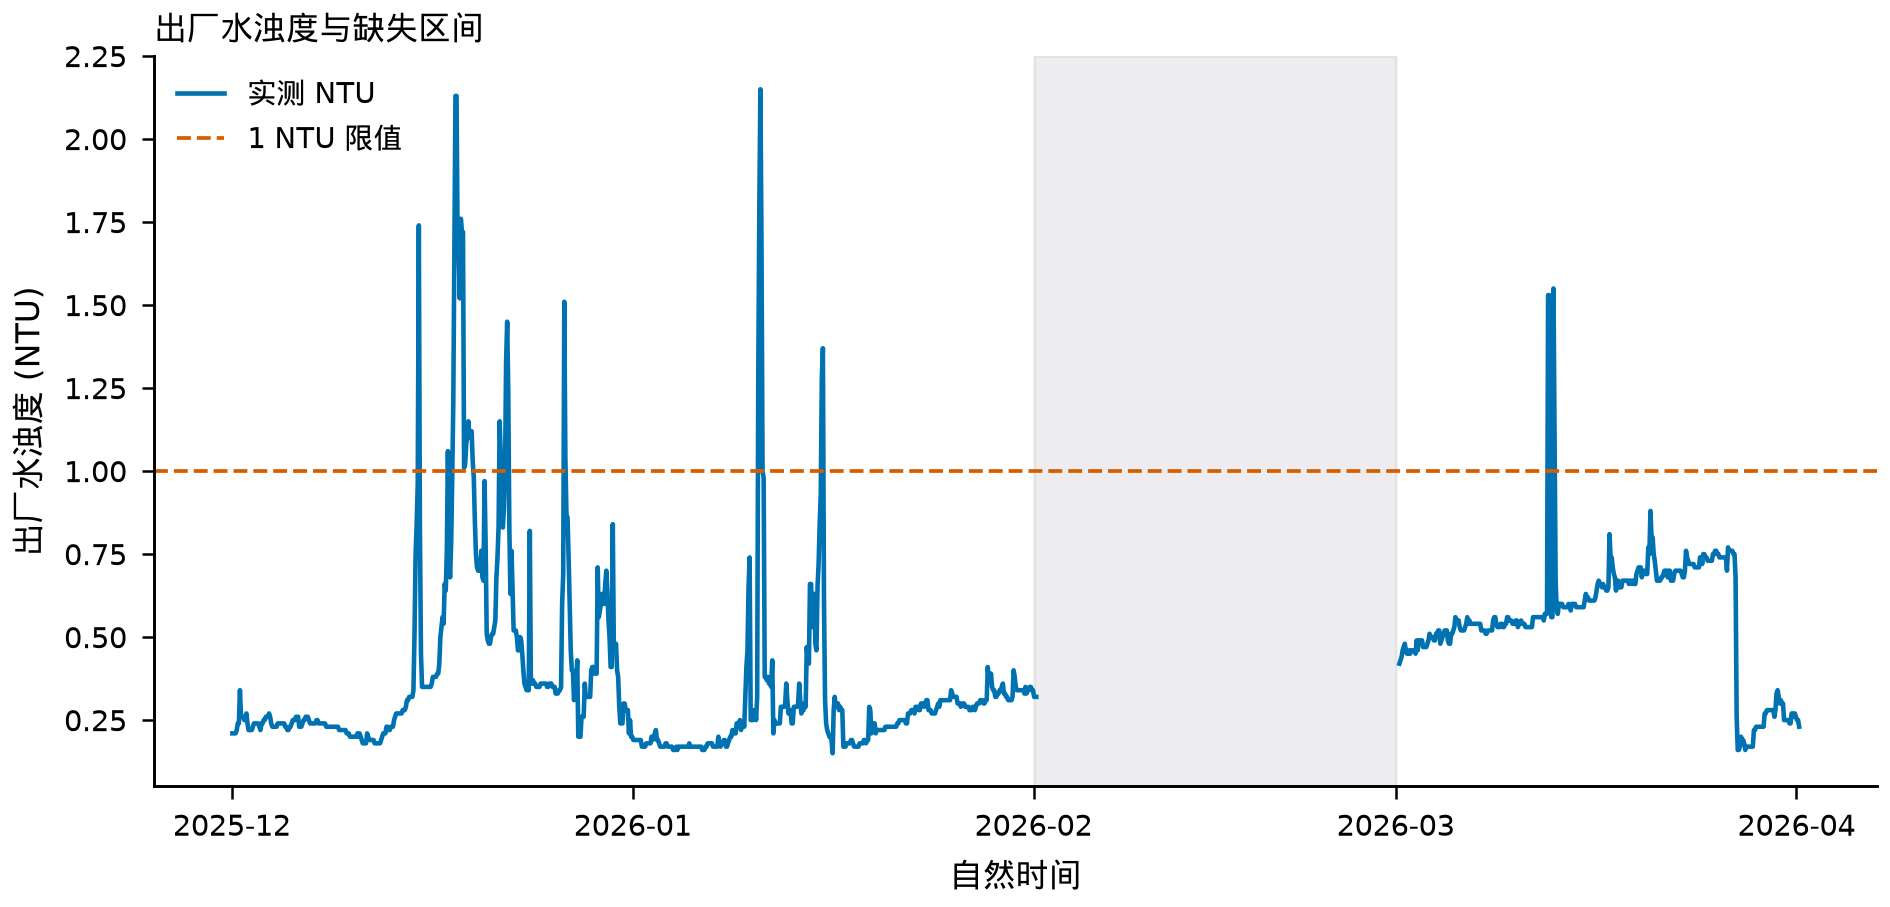
\includegraphics[width=0.88\textwidth]{raw_q1_target_missing.png}
\caption{出厂水浊度观测与 2026 年 2 月缺失区间}
\label{fig:q1-missing}
\end{figure}

\subsection{滚动验证与外部检验}

为避免未来信息泄漏，参数选择使用四个滚动折：训练端分别截止到 2025 年 9、10、11、12 月之前，验证端为随后一个月。2026 年 1 月用于问题一因素的后验检验，2026 年 3 月统一承担外部检验。评价指标为
\begin{equation}
\mathrm{RMSE}=\sqrt{\frac{1}{n}\sum_{i=1}^{n}(y_i-\hat y_i)^2},\qquad
\mathrm{MAE}=\frac{1}{n}\sum_{i=1}^{n}|y_i-\hat y_i|,
\label{eq:metrics1}
\end{equation}
\begin{equation}
\Rtwo=1-\frac{\sum_i(y_i-\hat y_i)^2}{\sum_i(y_i-\bar y)^2}.
\label{eq:metrics2}
\end{equation}
当 $\Rtwo<0$ 时，模型在该检验集上甚至弱于以检验集均值为预测的参照，必须作为失败证据报告。RMSE、MAE 与 $\Rtwo$ 的含义互补，单独报告无尺度背景的误差不足以判断回归质量\cite{chicco2021}。

滚动设计包含三层彼此隔离的用途。第一层是训练窗，用于拟合预处理器和系数；第二层是随后一个月，用于选择岭参数、时滞、自回归阶数或 RTD 时间尺度；第三层是未参加选择的 2026 年 3 月，用于最终外部评价。问题一的 2026 年 1 月因素筛选也不回流修改 2025 年训练模型。若在切分前对全期数据做标准化，二月和三月的分布信息会进入训练；若随机打乱两小时时点，强自相关又会使相邻样本同时落入训练和验证。本文在每个折内重新估计全部变换参数，从实现上排除这两类泄漏。

基线的设置同样遵循任务尺度。问题一使用“同营运时次前一日”预测，反映出厂浊度的日周期与短期稳定性；问题三对每个时距使用当前出厂水持续值，反映在线多步预测最容易获得的信息。只有模型在同一测试点、同一指标下超过对应基线，才可声称获得增量预测价值。训练期拟合优度、不同样本量下的误差或物理基线本身的解释性均不能替代这一比较。

\section{问题一：主要因素与条件预测}

\subsection{Huber 岭主模型}

设出厂水浊度为 $Y_t$。对原水浊度、原水色度和滤后水浊度使用 $g(x)=\log(1+x)$，其他连续变量使用恒等变换；每个变量加入当前值及 2、4、6、12 h 滞后。预处理后的特征为
\begin{equation}
z_{tj}=\frac{\operatorname{clip}(g_j(x_{tj}),l_j,u_j)-\mu_j}{s_j},
\label{eq:standardize}
\end{equation}
其中 $l_j,u_j$ 为训练集 0.5\% 和 99.5\% 分位数。主函数关系写为
\begin{equation}
\widehat Y_t=\max\left\{0,\exp\left(\beta_0+\sum_{j=1}^{59}\beta_jz_{tj}\right)-1\right\}.
\label{eq:q1function}
\end{equation}
系数通过带岭惩罚的 Huber M 估计得到。令残差的稳健标准化值为
\begin{equation}
u=\frac{e}{1.4826\operatorname{median}|e-\operatorname{median}(e)|},
\end{equation}
则其对应权重为
\begin{equation}
w(u)=\begin{cases}1,& |u|\le 1.345,\\1.345/|u|,& |u|>1.345.\end{cases}
\label{eq:huber}
\end{equation}
迭代 5 次，并在 $\{0.01,0.1,1,10,100\}$ 中滚动选择岭参数。稳健 M 估计与岭约束结合可同时降低异常响应和共线性的影响\cite{hampel1992,yasin2021}。为检查显著非线性，另用 256 个随机傅里叶特征近似高斯核并拟合岭回归；随机特征可把核岭问题转为有限维线性计算\cite{avron2017}。

Huber 岭的迭代可写为加权惩罚最小二乘。第 $r$ 次迭代根据上一次残差计算对角权重矩阵 $W^{(r)}$，再求
\begin{equation}
\boldsymbol\beta^{(r+1)}=arg\min_{\boldsymbol\beta}
\left\|{W^{(r)}}^{1/2}(\boldsymbol y-Z\boldsymbol\beta)\right\|_2^2
+\lambda\left\|\boldsymbol\beta_{-0}\right\|_2^2,
\label{eq:huber-ridge-objective}
\end{equation}
其中截距不受惩罚。所有响应计算均在 $\log(1+Y)$ 尺度完成，反变换后截断为非负值。岭项不是为了制造稀疏系数，而是稳定 59 个当前项与滞后项间的共线设计；主要因素的选择另由组置换完成。因此，不能简单按单个标准化系数绝对值排序：同一原始变量的五个时间项可能符号不同且高度相关，单系数既不能代表总贡献，也会随标准化尺度改变。

非线性对照先对同一标准化向量构造随机特征 $\varphi(z)$，再估计
\begin{equation}
\widehat y=\alpha_0+\boldsymbol\alpha^{\mathsf T}\varphi(z),\qquad
\varphi_k(z)=\sqrt{\frac{2}{256}}\cos(\boldsymbol\omega_k^{\mathsf T}z+b_k),
\end{equation}
其中 $b_k$ 在 $[0,2\pi]$ 上均匀生成，随机种子固定。其作用是检查主模型遗漏的平滑非线性是否能改善外部预测，而不是替代可解释的因素筛选。滚动选择得到 Huber 岭的 $\lambda=100$；RFF 对照的核尺度因子为 1、岭参数为 100，平均滚动 RMSE 为 0.683810 NTU。两套模型在预处理、时间切分和外部测试点上完全一致，故比较不受样本口径差异影响。

\subsection{分块置换和方向一致性}

因素贡献在 2026 年 1 月上计算。基准与置换预测严格共用仅训练至 2025 年末的同一个模型，把某原始变量及其全部滞后项按 24 h 块同步置换，定义
\begin{equation}
\Delta_j=\mathrm{RMSE}(Y,\widehat Y^{\mathrm{perm}(j)})-\mathrm{RMSE}(Y,\widehat Y).
\label{eq:perm}
\end{equation}
方向则以训练集中该变量从 25\% 分位数变到 75\% 分位数、其他特征固定在中位数时的条件响应差为准，并与各滚动折的 Spearman 符号比较。主要因素必须同时满足：$\Delta_j>0$、贡献排名前 6、四折方向一致率不低于 75\%。

采用 24 h 块而不是逐行随机置换，是因为水质序列存在日内连续性。逐点打乱会生成相邻两小时剧烈跳变的非真实输入，所得误差增量容易混入“破坏时间结构”的影响；块置换保留每块内部的 12 个两小时时次，只改变日块出现的顺序。每次置换同时移动某变量的当前项与全部滞后项，使 $\Delta_j$ 衡量变量组的信息，而不是把相同来源的特征相互当作替代品。若置换后 RMSE 不升反降，则说明该组在检验期没有稳定增量信息，即使训练系数较大也不入选。

方向一致性是第二道约束。条件效应比较四分位点间的预测差，Spearman 系数则直接描述原变量和响应的单调关联；二者在受控和未受控口径下回答不同问题。本文要求滚动折中二者符号具有稳定支持，并同时查看相关系数的区间。这样做会牺牲“发现更多变量”的表面丰富性，却降低偶然月份、共线替代或控制策略变化造成的错误解释。

图~\ref{fig:q1-factor} 表明，只有滤后水浊度和原水色度通过全部门槛。滤后水浊度的 $\Delta=0.115354$ NTU，四折方向均为正；原水色度的 $\Delta=0.024035$ NTU，四折方向均为负。二者的 25\% 到 75\% 条件效应分别为 $+0.058381$ 和 $-0.050115$ NTU。负向色度关系可能来自投药和工况共同调节，不能解释为提高原水色度会直接降低出厂浊度。

\begin{figure}[htbp]
\centering
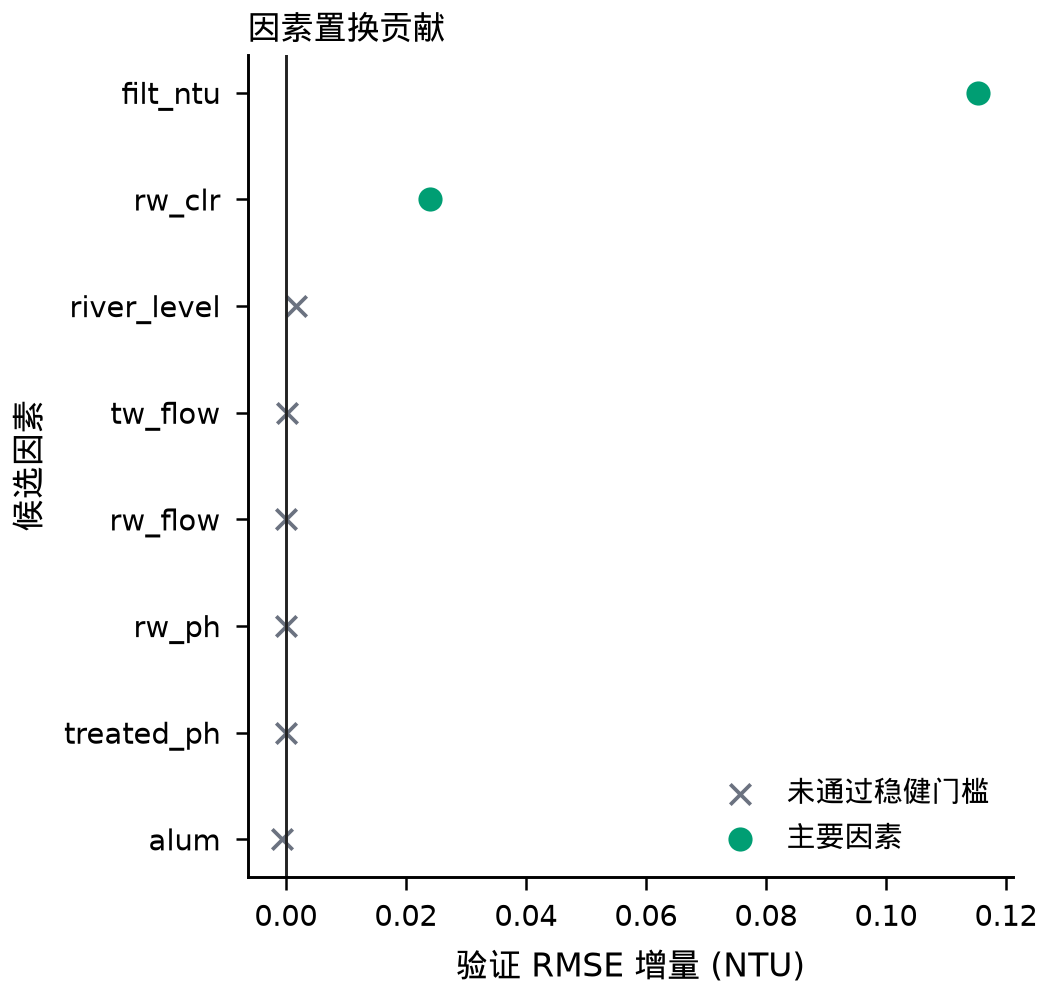
\includegraphics[width=0.53\textwidth]{process_q1_factor_screening.png}
\caption{时间块置换贡献与稳健因素筛选}
\label{fig:q1-factor}
\end{figure}

完整函数由式~\eqref{eq:q1function} 与 60 行参数表共同确定。表~\ref{tab:q1factor} 给出主要因素的汇总；所有当前项和滞后项系数、缩尾上下界、中心与尺度均保存在结果工作簿的“Q1函数参数”工作表中，单变量条件响应保存在“Q1偏效应”工作表中。

\begin{table}[htbp]
\centering
\caption{问题一主要因素筛选结果}
\label{tab:q1factor}
\begin{tabular}{lrrrr}
\toprule
因素 & 置换 RMSE 增量 & 条件效应 & Spearman $\rho$ & 四折一致率\\
\midrule
滤后水浊度 & 0.115354 & 0.058381 & 0.261720 & 1.00\\
原水色度 & 0.024035 & $-0.050115$ & $-0.113802$ & 1.00\\
\bottomrule
\end{tabular}
\end{table}

\subsection{指定日条件预测和外部失败证据}

图~\ref{fig:q1-forecast} 给出 2 月 1、10、20 日各 12 个营运时点的中心预测与滚动残差 95\% 区间。三个营运日中心值大致位于 0.15--0.35 NTU，而区间上界普遍超过 1 NTU。例如 2 月 10 日 13:00 的中心值为 0.354851 NTU，区间为 0.117044--1.782331 NTU。宽区间来自跨月份残差分布，体现了整月目标缺失下不可消除的不确定性。

\begin{figure}[htbp]
\centering
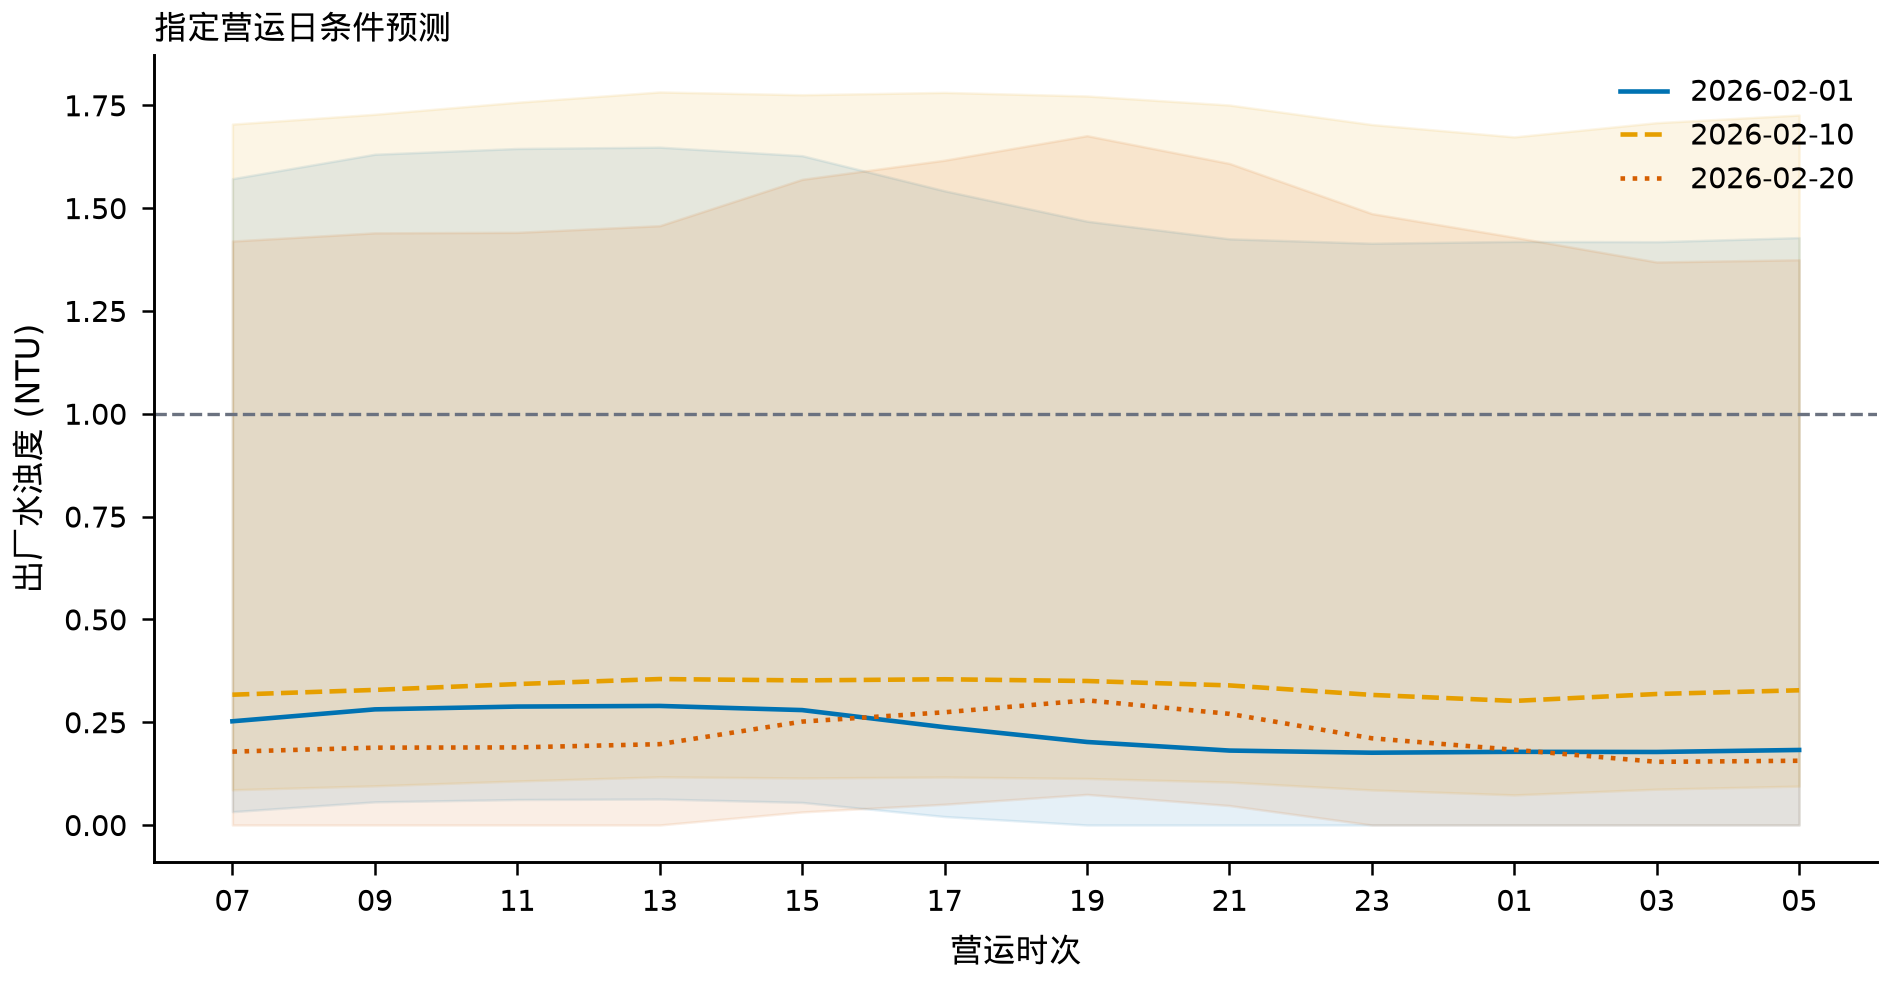
\includegraphics[width=0.88\textwidth]{result_q1_february_predictions.png}
\caption{三个指定营运日的出厂水浊度条件预测及 95\% 区间}
\label{fig:q1-forecast}
\end{figure}

表~\ref{tab:q1eval} 是必须与图~\ref{fig:q1-forecast} 同时阅读的外部检验。Huber 岭和 RFF 岭的 3 月 $\Rtwo$ 均为显著负值，同营运时次前一日基线的 RMSE 反而最低。故本文不声称问题一模型可以跨月泛化，2 月曲线只是在给定同期上游和运行变量条件下的估计。

预测区间由滚动验证残差构造。对每个二月时点先得到条件中心，再在对数尺度叠加来自历史验证窗的经验残差分位数，最后反变换到 NTU 尺度。该区间同时包含常态噪声、月份间模型偏差和部分未观测工况差异，因此明显不对称；它不是仅由回归系数标准误得到的窄置信带。由于二月没有目标观测，无法检验该月 95\% 区间是否真正达到 95\% 覆盖，故文中只称其为基于历史滚动残差的预测区间，不作校准完成的承诺。

从外部误差结构看，Huber 岭 RMSE 0.392112 NTU，约为前一营运日基线 0.170873 NTU 的 2.30 倍；RFF 岭 RMSE 也约为基线的 2.17 倍。非线性对照相对主模型只减少约 0.0205 NTU 的 RMSE，远不足以弥合与简单基线的差距，说明问题不只是线性形式过于简单。更可能的原因包括二月目标整段缺失导致无法校准近期偏移、三月存在训练期少见的状态，以及条件变量的缺失和投药闭环削弱了稳定映射。基于这些证据，指定日结果适合用于“在已知同期变量下大致处于何种范围”的辅助研判，不适合用于替代在线浊度仪、承诺合格或反推单一变量的控制动作。

两个入选因素也应作过程化解释。滤后水位于出厂水上游，其正向条件效应与颗粒物经过清水池后仍保留部分变化相符；原水色度的负向条件效应则很可能混合了混凝剂调整、原水来源和季节工况。当原水色度升高时，操作人员可能同步增强处理，使出厂浊度并不按未经控制的方向变化。这正是观察数据中的“受策略调节关联”，而不是原水色度本身具有降低浊度的物理作用。论文因此报告效应大小、符号稳定性和相关区间，却避免使用“决定”“导致”等因果措辞。

\begin{table}[htbp]
\centering
\caption{问题一 2026 年 3 月外部检验}
\label{tab:q1eval}
\begin{tabular}{lrrr}
\toprule
模型 & RMSE/NTU & MAE/NTU & $\Rtwo$\\
\midrule
Huber 岭 & 0.392112 & 0.345015 & $-3.447487$\\
RFF 岭 & 0.371614 & 0.318837 & $-2.994651$\\
同营运时次前一日 & 0.170873 & 0.065256 & 0.173359\\
\bottomrule
\end{tabular}
\end{table}

\section{问题二：滤后水动态响应和有效时滞}

\subsection{ARX-Ridge 结构}

图~\ref{fig:q2-series} 显示原水与滤后水浊度相差一个至多个数量级，且滤后水偶尔出现尖峰。因此对两者使用对数尺度。设滤后水浊度为 $F_t$，四个外生输入为原水浊度、原水 pH、混凝剂投加量和原水流量，模型为
\begin{equation}
\log(1+F_t)=a_0+\sum_{k=1}^{p}\phi_k\log(1+F_{t-k})+
\sum_{m=1}^{4}h_m(X_{m,t-d_m})+\epsilon_t,
\label{eq:arx}
\end{equation}
其中 $h_m$ 包含一次项和平方项，并加入原水浊度与混凝剂、pH 与混凝剂的交互项。$d_m$ 独立取 0、2、4、6 h，先对 $4^4=256$ 个组合和 5 个岭值做滚动搜索，再在 $p\in\{3,6,9,12\}$ 中选择自回归阶数。

该结构把两类动态分开：$\phi_k$ 描述滤后水自身的惯性和未显式观测的慢变化，$d_m$ 与 $h_m$ 描述外生输入在候选延迟后的条件贡献。平方项允许输入在高、低区间具有不同斜率，两个交互项分别表示原水颗粒负荷与投药、酸碱状态与投药可能存在的协同变化。所有多项式项都在基础变量完成训练窗标准化后生成，以防平方项的量级主导惩罚。岭惩罚同时作用于自回归和外生系数，截距仍不惩罚。

对给定的 $\boldsymbol d=(d_1,\ldots,d_4)$、$p$ 和 $\lambda$，目标函数为
\begin{equation}
\min_{\boldsymbol\theta}\sum_{t\in\mathcal T}
\left[\log(1+F_t)-\boldsymbol z_t(\boldsymbol d,p)^{\mathsf T}\boldsymbol\theta\right]^2
+\lambda\|\boldsymbol\theta_{-0}\|_2^2.
\label{eq:arx-objective}
\end{equation}
候选时滞搜索先固定基础自回归结构，对 256 个组合分别考察 5 个岭值，共形成 1280 条验证记录；随后在选定时滞上比较 3、6、9、12 阶。这个顺序控制了计算规模，也使输入延迟与输出记忆长度的含义相对清楚。若一次性在所有阶数、交互形式和时滞上无约束搜索，有限的四个验证月容易选择到偶然最低点。

\begin{figure}[htbp]
\centering
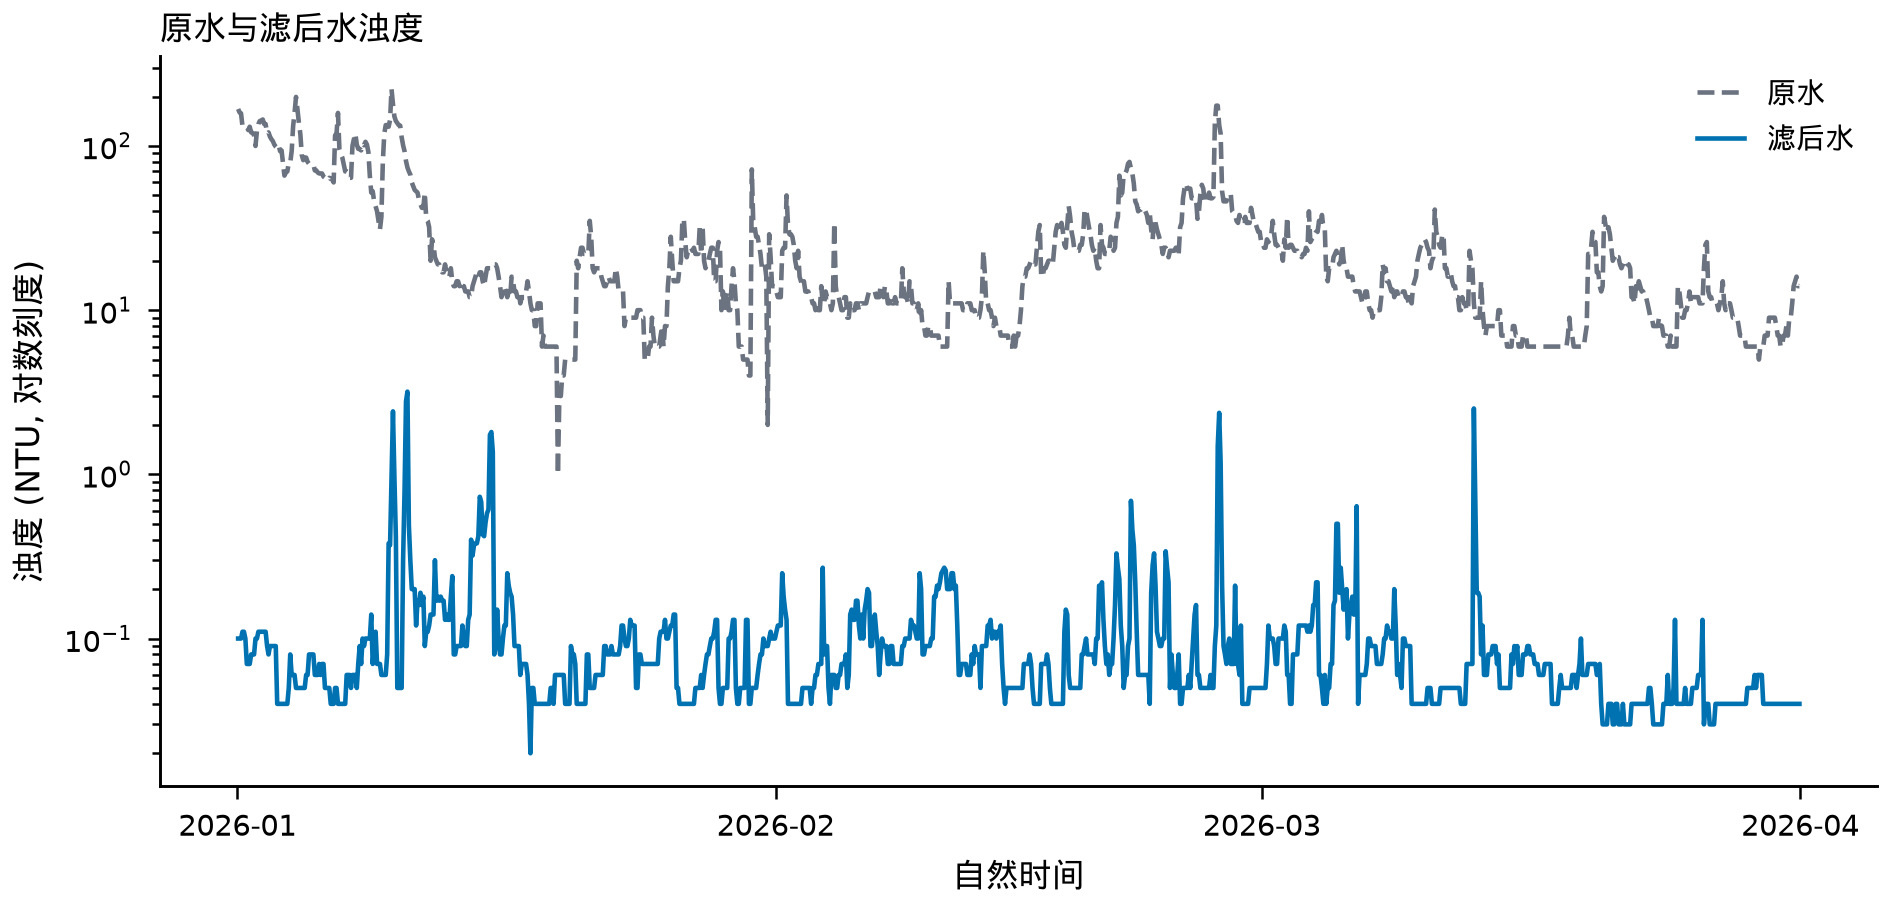
\includegraphics[width=0.88\textwidth]{raw_q2_input_output_series.png}
\caption{2026 年 1--3 月原水与滤后水浊度序列}
\label{fig:q2-series}
\end{figure}

\subsection{时滞结果与可辨识性}

图~\ref{fig:q2-lag} 把另外两个输入和岭值取最优后，展示原水浊度与混凝剂时滞组合的滚动误差。完整搜索保留 1280 行结果，没有用单变量相关峰替代多变量枚举。最优输入时滞为原水浊度 2 h、原水 pH 0 h、混凝剂 0 h、原水流量 6 h，岭为 0.01，自回归阶数为 6。对差分并预白化后的输入和目标作 0--12 h 互相关检查，峰值与 ARX 时滞差均不超过 4 h，故把它们记为数据支持的“有效时滞”。它们仍受控制策略和变量共线影响，不应直接等同于唯一物理输运时间。

如表~\ref{tab:q2lag} 所示，四个变量的互相关峰值绝对量仅为 0.0139--0.0408，说明单变量线性滞后信号很弱。原水浊度的 ARX 时滞为 2 h，而预白化互相关峰在 0 h；原水流量对应 6 h 与 2 h。两者之差仍位于预设的 4 h 可辨识容差内，但不能把 2 h 或 6 h 解读为精确到小时的水力停留时间。pH 和混凝剂选择 0 h，可能同时反映同一班次内的操作响应：观测到原水变化后立即调节投药，使输入与滤后响应在两小时采样网格上落入同一时次。

\begin{figure}[htbp]
\centering
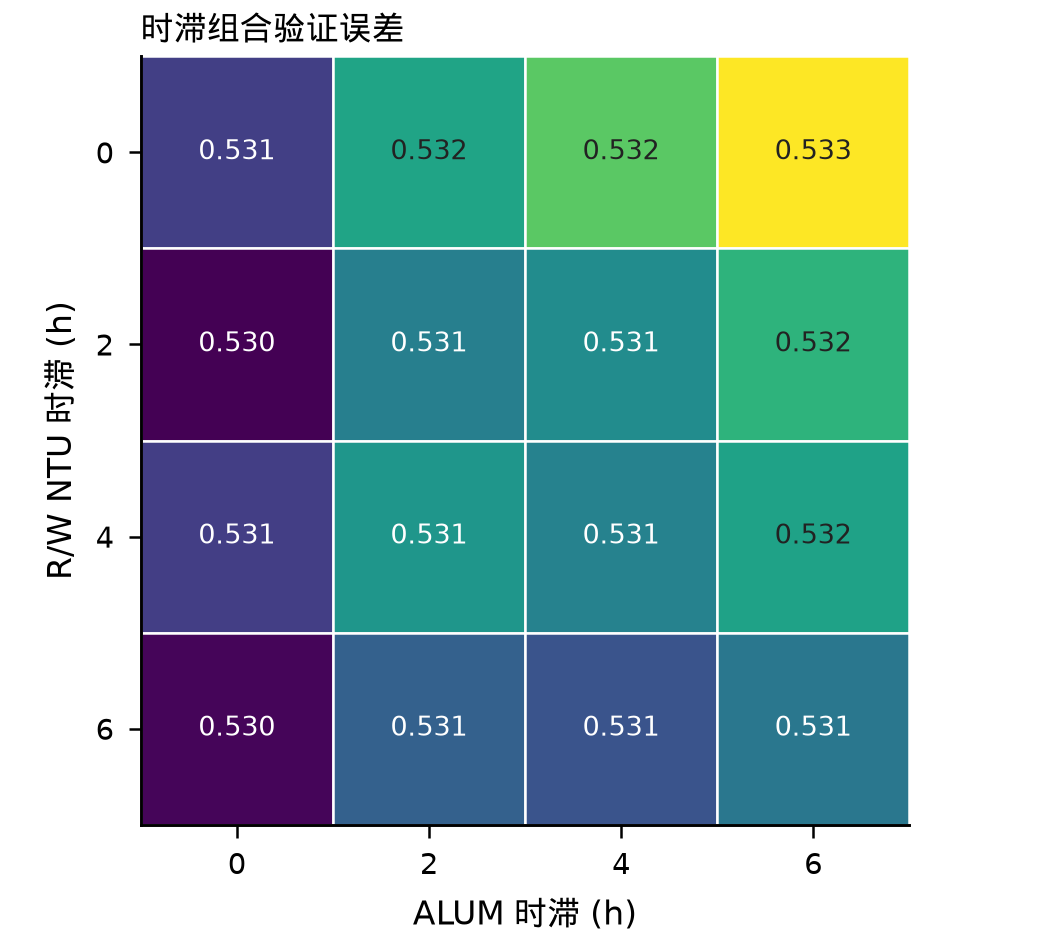
\includegraphics[width=0.53\textwidth]{process_q2_lag_search.png}
\caption{原水浊度与混凝剂时滞组合的最小滚动验证 RMSE}
\label{fig:q2-lag}
\end{figure}

\begin{table}[htbp]
\centering
\caption{问题二时滞与交叉相关检查}
\label{tab:q2lag}
\begin{tabular}{lrrrr}
\toprule
输入 & ARX 时滞/h & 互相关峰/h & 峰值相关 & 可辨识\\
\midrule
原水浊度 & 2 & 0 & 0.02443 & 是\\
原水 pH & 0 & 2 & 0.01392 & 是\\
混凝剂 & 0 & 0 & 0.02919 & 是\\
原水流量 & 6 & 2 & 0.04076 & 是\\
\bottomrule
\end{tabular}
\end{table}

\subsection{外部检验和残差诊断}

3 月外部检验 RMSE 为 0.166450 NTU、MAE 为 0.029398 NTU、$\Rtwo=-0.373590$。图~\ref{fig:q2-validation} 表明模型能跟随大部分低值水平，却不能稳定捕捉 3 月中旬的孤立尖峰。Ljung--Box 12 阶统计量为 72.3939，$p=1.14\times10^{-10}$；残差 1--6 阶最大绝对 ACF 为 0.416470。提高到 9 或 12 阶并未从滚动误差上获得足够收益，因此保留 6 阶并如实报告剩余相关性，而不是用更高阶数掩盖诊断失败。

RMSE 与 MAE 的明显差距揭示了误差的非均匀性：RMSE 约为 MAE 的 5.66 倍，少数大误差对平方损失贡献很高。若模型在所有时点都同等偏离，二者不会出现如此大的比例。结合外部检验图可知，常态低浊度段的大多数绝对误差较小，而尖峰的幅度或发生时刻未被正确预测。负 $\Rtwo$ 并不否定模型对常态水平的跟随能力，但表示在三月总体平方误差口径下，其增量解释不足。

自回归阶数敏感性进一步支持保守选择。固定最优时滞和 $\lambda=0.01$ 时，3、6、9、12 阶的平均滚动 RMSE 分别为 0.530303、0.529050、0.529913 和 0.529717 NTU。6 阶相对 3 阶仅改善 0.001254 NTU，相对 9 阶也只低 0.000863 NTU；阶数增加并未带来单调收益。岭参数从 0.01 增到 100 时，各阶误差均上升到约 0.542--0.545 NTU，说明过强收缩会损失已经很弱的动态信号。最终的 6 阶代表 12 h 输出历史，是滚动标准下的最小值，而不是声称滤池过程恰好只记忆 12 h。

Ljung--Box 检验的原假设是所检查滞后内残差不相关。极小的 $p$ 值与 0.416470 的最大绝对自相关共同拒绝该假设，意味着标准独立误差假定不成立。剩余相关可能来自反冲洗、滤池组切换、在线仪表滞后或未记录的降雨事件；这些信息在现有字段中不可辨识。因而本模型适合给出“在现有输入与历史状态下的条件平均响应”，不适合把残差当白噪声直接生成独立逐点置信区间。后续问题三使用成块的多时距误差重采样，正是为了避免继续采用独立误差假设。

从营运角度看，时滞结果可以用于安排观测窗口，而不能直接用于自动投药。例如原水流量的有效延迟为 6 h，提示评估某次流量变化时不宜只检查当前滤后水；原水浊度的 2 h 延迟则提示较快响应。但由于交叉相关很低、外部 $\Rtwo$ 为负，任何基于这些延迟的控制策略都应先在更多事件期验证。特别是混凝剂与滤后浊度之间存在反向调节闭环，不能据回归系数直接计算“增加多少药剂必然降低多少浊度”。

\begin{figure}[htbp]
\centering
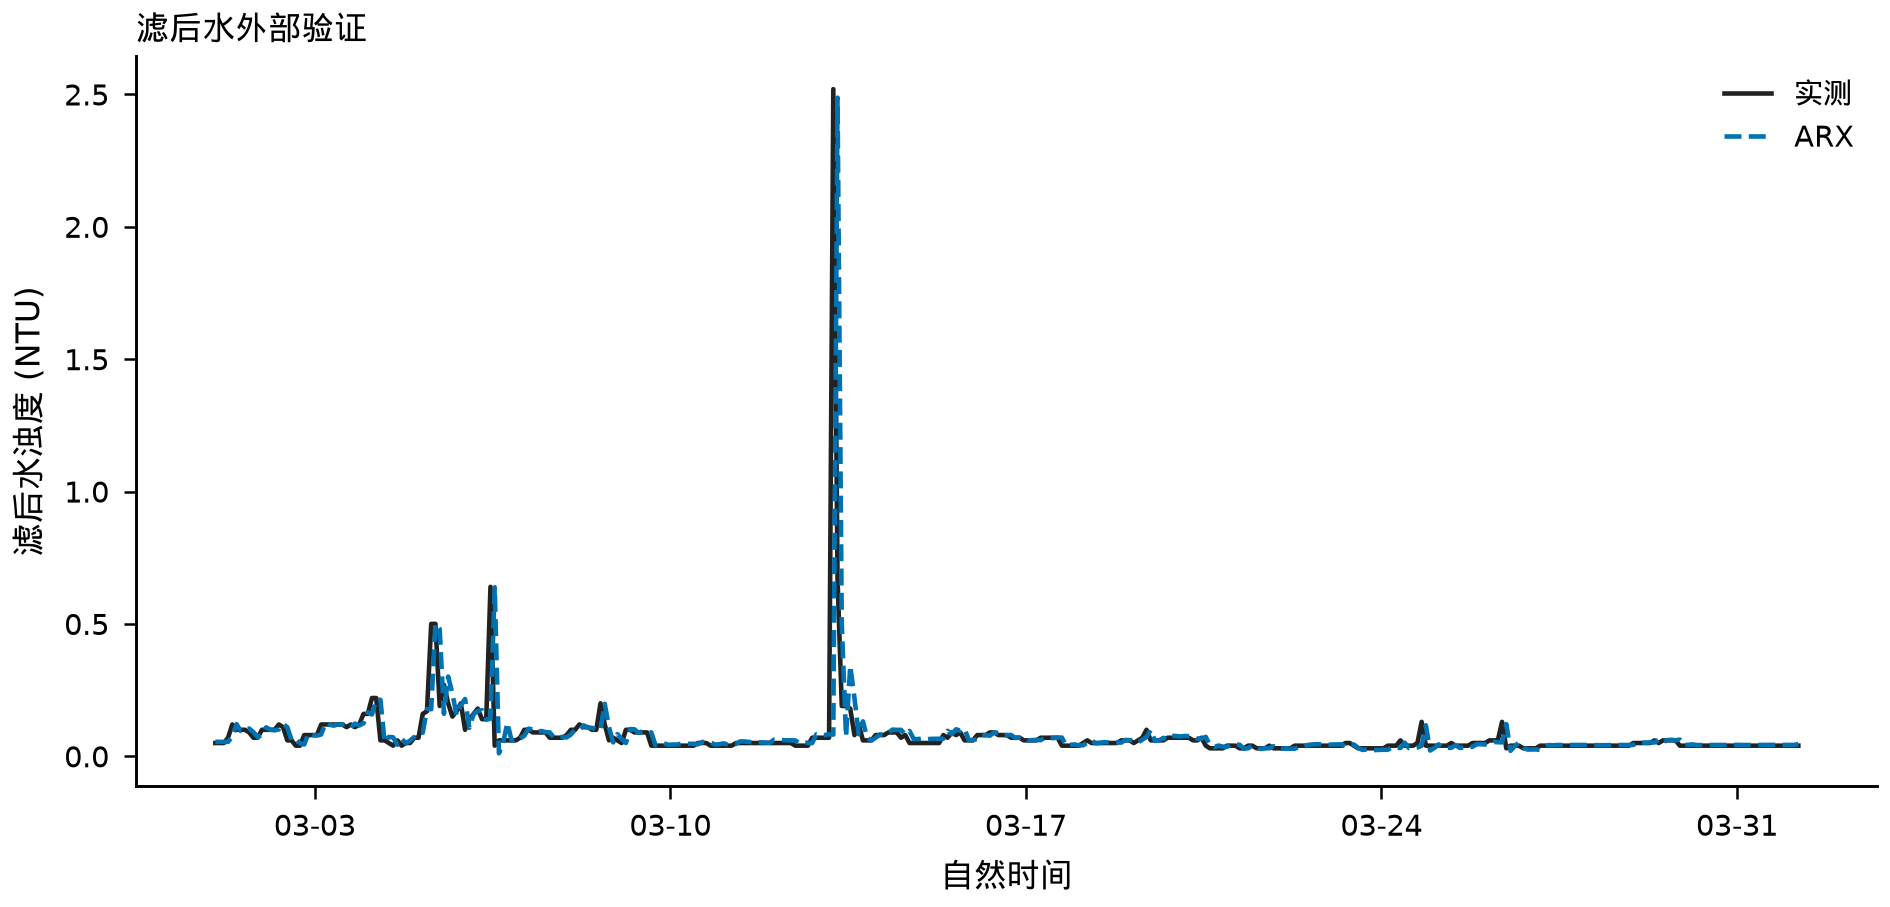
\includegraphics[width=0.88\textwidth]{result_q2_external_validation.png}
\caption{ARX-Ridge 对滤后水浊度的 2026 年 3 月外部检验}
\label{fig:q2-validation}
\end{figure}

\section{问题三：清水池传播与 1--12 h 预测}

\subsection{质量守恒的停留时间分布}

图~\ref{fig:q3-propagation} 显示清水池前后的短期波动并非简单平移。本文以指数停留时间分布作为连续搅拌近似；指数 RTD 是单个理想连续搅拌槽的基本情形，并具有滤除上游高频波动的解释\cite{toson2019}。令采样间隔 $\Delta t=2$ h，$q=\exp(-\Delta t/\tau)$，截取累计质量不低于 95\% 的 $J$ 项并重新归一化：
\begin{equation}
k_j=\frac{q^j}{\sum_{r=0}^{J-1}q^r},\quad j=0,\ldots,J-1,
\qquad P_t=\sum_{j=0}^{J-1}k_jF_{t-j}.
\label{eq:rtd}
\end{equation}
由此严格满足 $\sum_jk_j=1$。在 $\tau=2,4,\ldots,24$ h 中滚动选择，得到 $\tau=8$ h。图~\ref{fig:q3-rtd} 左侧给出离散核，右侧给出各候选尺度的验证误差。

核的非负性与单位质量具有直接含义：若一段时间内所有滤后水浊度都等于常数 $c$，则 $P_t=c$，传播层不会无故放大或缩小常值水平。对 $\tau=8$ h 和 $\Delta t=2$ h，有 $q=\exp(-0.25)\approx0.7788$，较近的滤后水获得较大权重，较远历史按几何速度衰减。截断点由累计质量 95\% 决定，截断后再次归一化，因此数值核质量为 1.0。该步骤消除了有限记忆窗口造成的系统性质量损失。

$\tau$ 是“有效混合时间尺度”，并非直接测得的池体容积除以流量。它综合了池内混合、采样频率以及滤后和出厂监测位置间的相对响应。候选值从 2 h 到 24 h 以 2 h 递增，与数据分辨率一致；过小的 $\tau$ 使 $P_t$ 接近当前滤后值，过大的 $\tau$ 会过度平滑并引入很长历史。滚动验证选择 8 h 表示在现有候选与损失函数下取得最低误差，而不是证明池体服从唯一指数分布。

\begin{figure}[htbp]
\centering
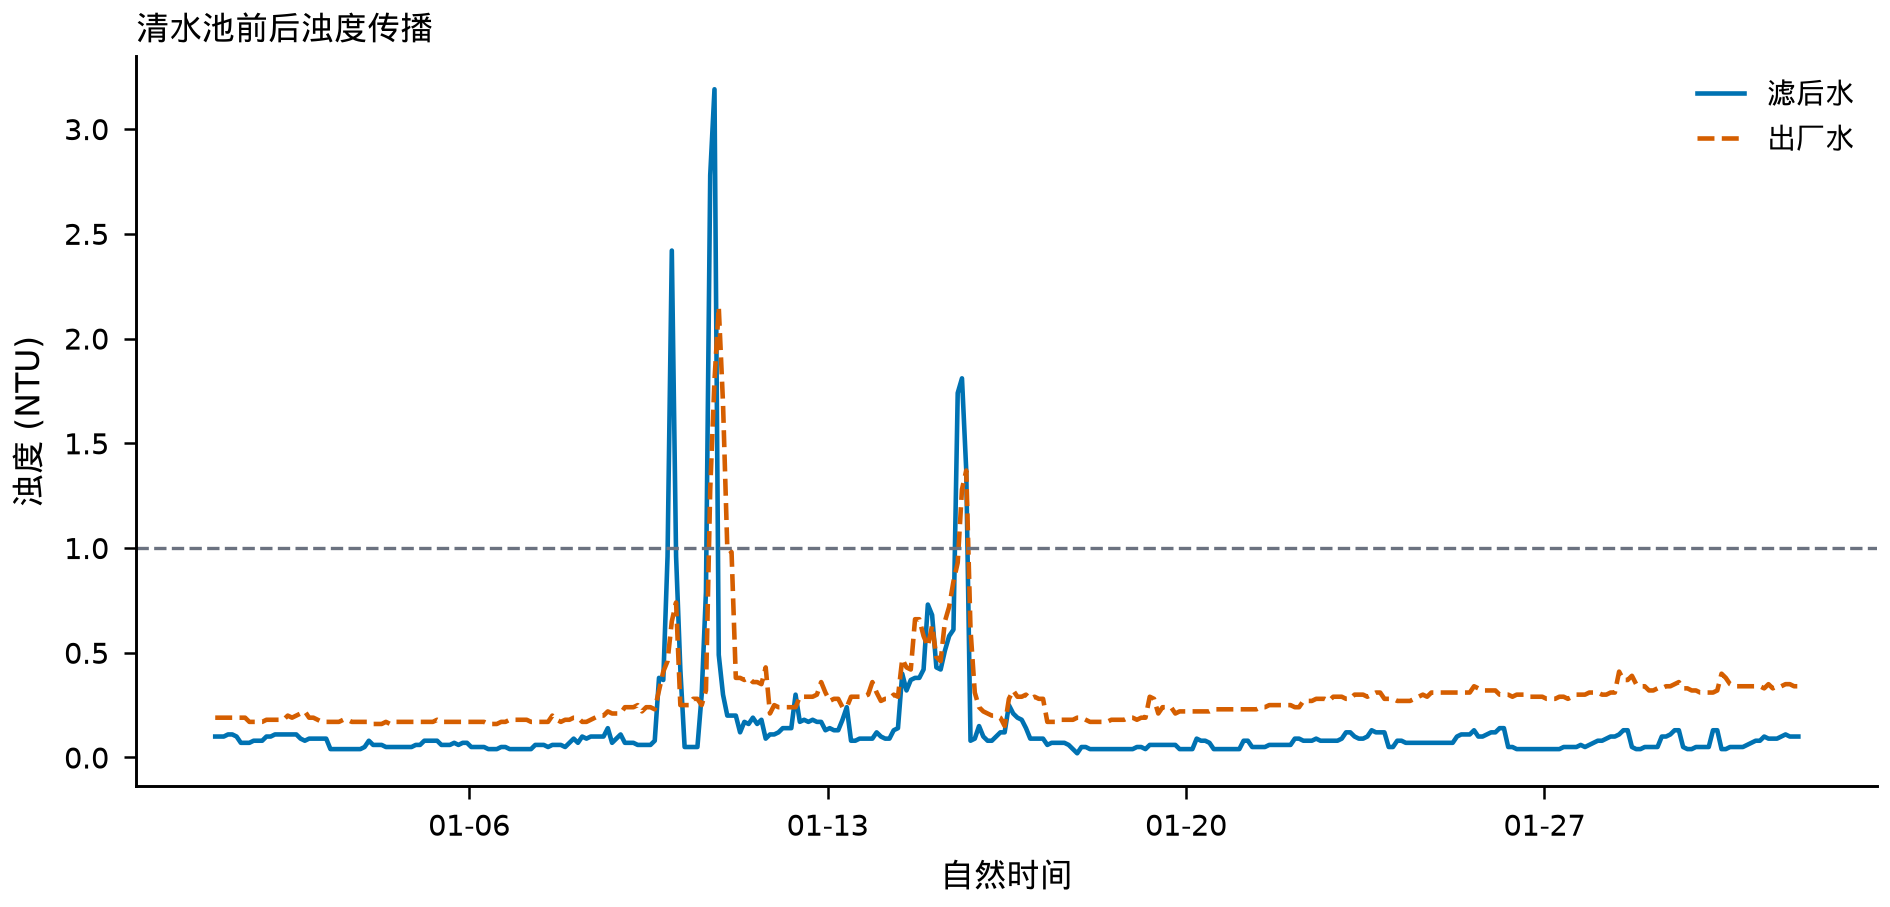
\includegraphics[width=0.88\textwidth]{raw_q3_filtered_treated_series.png}
\caption{2026 年 1 月清水池前后浊度传播}
\label{fig:q3-propagation}
\end{figure}

\begin{figure}[htbp]
\centering
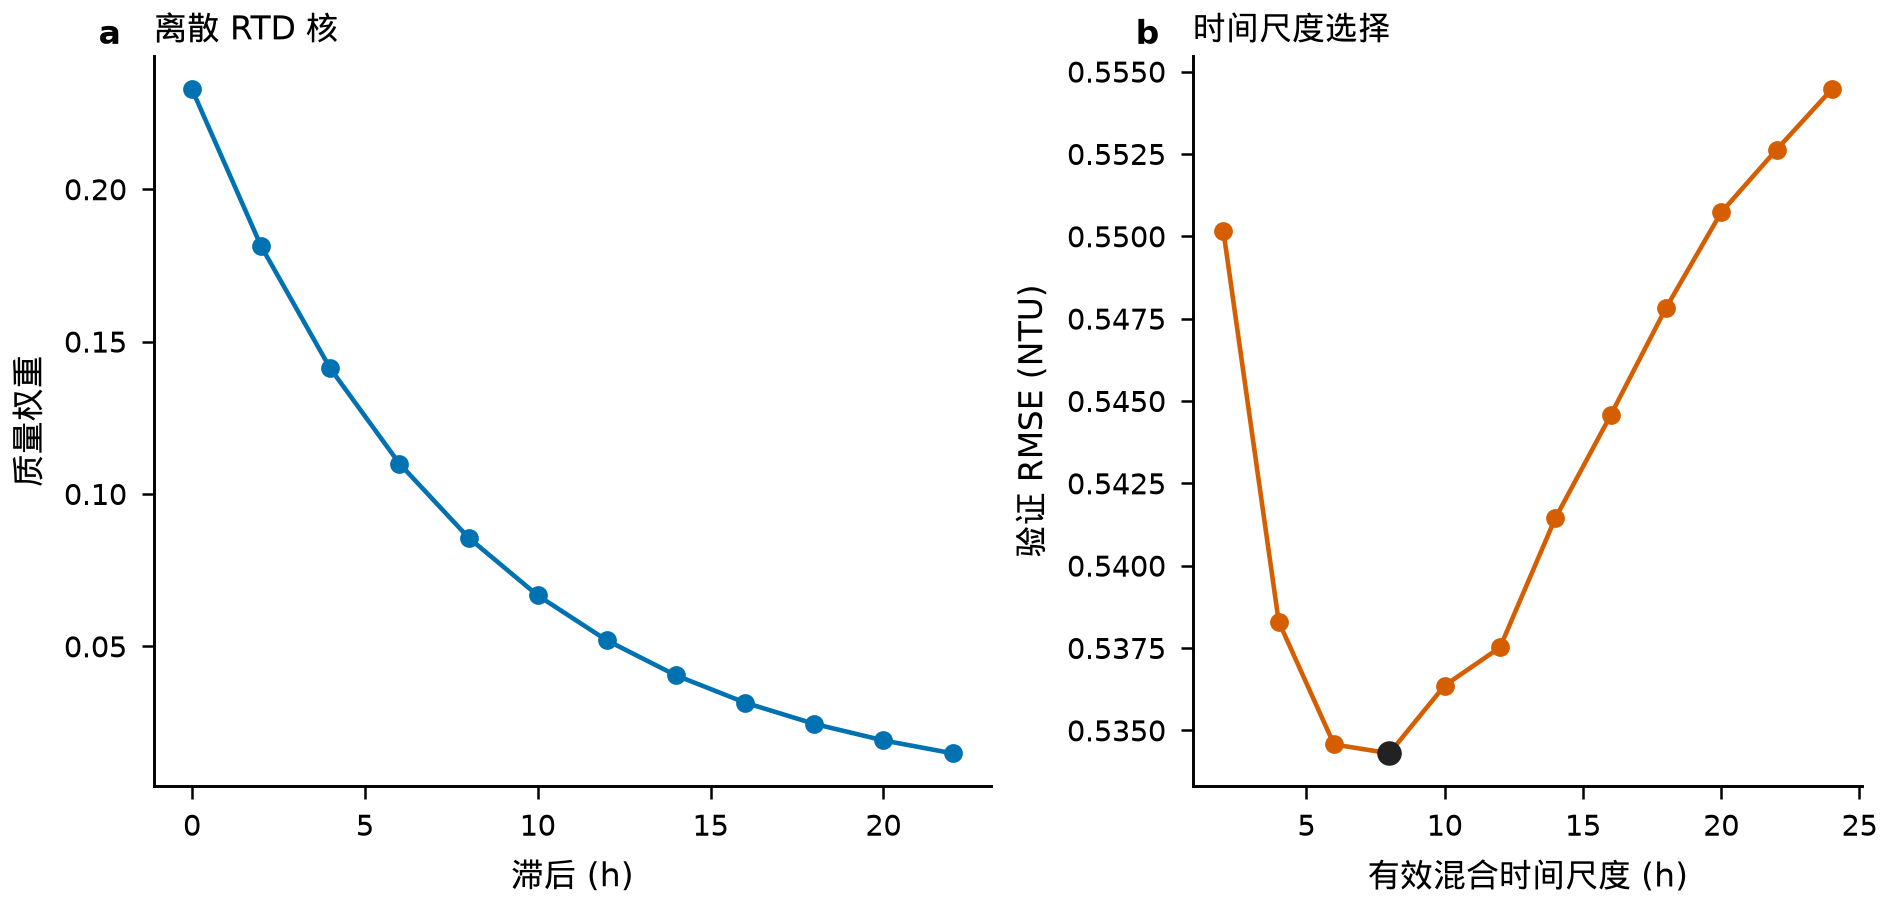
\includegraphics[width=0.88\textwidth]{process_q3_rtd_selection.png}
\caption{指数 RTD 核及有效混合时间尺度选择}
\label{fig:q3-rtd}
\end{figure}

\subsection{对数残差修正和联合轨迹}

纯 RTD 基线不能表达投药、流量与短期状态的偏离。定义 $R_t=\log(1+Y_t)-\log(1+P_t)$，对每个偶数时距 $h\in\{2,4,6,8,10,12\}$ 分别建立
\begin{equation}
\log(1+\widehat Y_{t+h})=\log(1+P_{t+h})+f_h
\left(R_t,\ldots,R_{t-10\mathrm{h}},U_t\right),
\label{eq:hybrid}
\end{equation}
其中 $U_t$ 包含原水浊度、滤后水浊度、混凝剂、原水和出厂流量以及时次正余弦项，$f_h$ 为滚动选择岭值的 Huber 回归。

残差层选择对数尺度有两点原因。一是浊度非负且偶有高值，直接相加的误差在高、低水平下方差差异明显；二是 $R_t$ 表示观测出厂水相对物理基线的比例型偏离，反变换后仍可通过零下截断维持可行域。时次的正余弦编码为
\begin{equation}
c_t=\cos\left(2\pi s_t/12\right),\qquad
s_t^{\ast}=\sin\left(2\pi s_t/12\right),
\end{equation}
其中 $s_t=0,\ldots,11$ 表示营运日内时次。循环编码使 05:00 与下一营运日 07:00 在特征空间连续，不会因整数编码首尾相距 11 而产生伪距离。

六个偶数时距采用直接预测而非把 2 h 模型反复迭代到 12 h。直接模型允许不同 $h$ 使用不同系数和岭强度，避免单步偏差机械累积；选得的岭参数按 2、4、6、8、10、12 h 依次为 1、1、10、10、1、1。另一方面，二月完整轨迹生成仍需随时间推进，因此在每个新时点把模拟出的 $Y$ 写回最近残差状态。这形成“直接时距校正 + 逐时轨迹递推”的组合：前者服务于各预测时距的回测，后者保证整月风险评价拥有时间上连续且内部相关的样本路径。

为保留不同预测时距误差之间的相关性，从 2026 年 1 月滚动回测中组成 6 维误差向量，再按 12 个起点为一块进行移动块重采样。移动块自助法能够在重采样时保留时间依赖，适合水文参数与预测不确定性分析\cite{ebtehaj2010}。固定种子 20260727 生成 500 条联合递推轨迹；每一步把上一步模拟出厂水写回残差状态，因此二月的不确定性会随递推传播，而非把逐时独立区间拼接成轨迹。

设第 $b$ 条重采样路径在起点 $t$ 获得六维误差向量 $\boldsymbol e_t^{(b)}$，则偶数时距模拟值写为
\begin{equation}
Y_{t+h}^{(b)}=\max\left\{0,
\exp\left[\widehat\eta_{t,h}+e_{t,h}^{(b)}\right]-1\right\},
\qquad b=1,\ldots,500,
\label{eq:path}
\end{equation}
其中 $\widehat\eta_{t,h}$ 是式~\eqref{eq:hybrid} 的确定部分。块长 12 个起点对应约一个营运日，既保留日内连续误差，也允许跨块组合不同历史片段。每个时点的 2.5\%、50\% 和 97.5\% 分位数形成点预测区间；问题四则不先取分位数，而是对每一条完整路径独立计算日指标和等级，以保留非线性分级的真实顺序。

500 条路径是在计算稳定性与结果规模间的折中。路径数过少会使 2.5\% 尾部分位数只由极少样本决定，过多则显著增加整月递推和工作簿存储。固定随机种子保证相同输入和代码下的等级概率、区间上下界逐次一致，但它不意味着随机误差本身消失。若用于正式风险控制，应通过改变种子和路径数检查 Monte Carlo 稳定性，并在新观测到达后滚动更新残差块库。

\subsection{分时距结果和解释边界}

表~\ref{tab:q3acc} 与图~\ref{fig:q3-accuracy} 给出 3 月滚动起点回测。混合模型在 2、4、6、8、10 h 均未超过持续性，只有 12 h 的 RMSE 0.139042 略小于持续性的 0.142469。纯物理基线 RMSE 约 0.52--0.54 NTU，说明 RTD 更适合作为结构基线而非独立精确预测器。混合模型区间覆盖率为 0.967--0.978，虽接近或高于 95\%，但不能脱离区间宽度解释为高精度。

分时距比较揭示了两种误差来源。2 h 时持续性 RMSE 为 0.092239 NTU，混合模型为 0.097030 NTU，差值仅 0.004791 NTU，表明出厂水短期惯性已很强，复杂特征没有提供稳定增益。到 8 h，二者差距扩大到 0.016773 NTU，混合修正仍未胜出。12 h 时混合模型比持续性低 0.003427 NTU，相对改善约 2.41\%，属于小幅而非决定性优势。故不能用“最长时距获胜”概括为全时距优于基线。

尽管绝对误差比较并不占优，混合模型在外部回测的 $\Rtwo$ 仍为 0.344--0.728，说明它能解释三月部分时序变化。这与 RMSE 基线结果并不矛盾：$\Rtwo$ 是相对检验集均值的比较，而持续性利用当前真实值，通常比均值强得多。实际在线预测应优先采用更严格的持续性基线比较。区间覆盖率高于名义 95\% 约 1.7--2.8 个百分点，可能表示区间略保守；在高后果水质场景中保守区间可以接受，但仍需同时报告宽度并用更多外部月份检验。

\begin{table}[htbp]
\centering
\caption{问题三分时距外部回测}
\label{tab:q3acc}
\begin{tabular}{rrrrr}
\toprule
时距/h & 混合 RMSE & 持续性 RMSE & 混合 $\Rtwo$ & 95\%覆盖率\\
\midrule
2 & 0.097030 & 0.092239 & 0.727982 & 0.9757\\
4 & 0.136679 & 0.131063 & 0.460999 & 0.9703\\
6 & 0.150911 & 0.137517 & 0.343940 & 0.9675\\
8 & 0.142009 & 0.125236 & 0.420173 & 0.9783\\
10 & 0.125370 & 0.120492 & 0.549029 & 0.9755\\
12 & 0.139042 & 0.142469 & 0.446533 & 0.9672\\
\bottomrule
\end{tabular}
\end{table}

\begin{figure}[htbp]
\centering
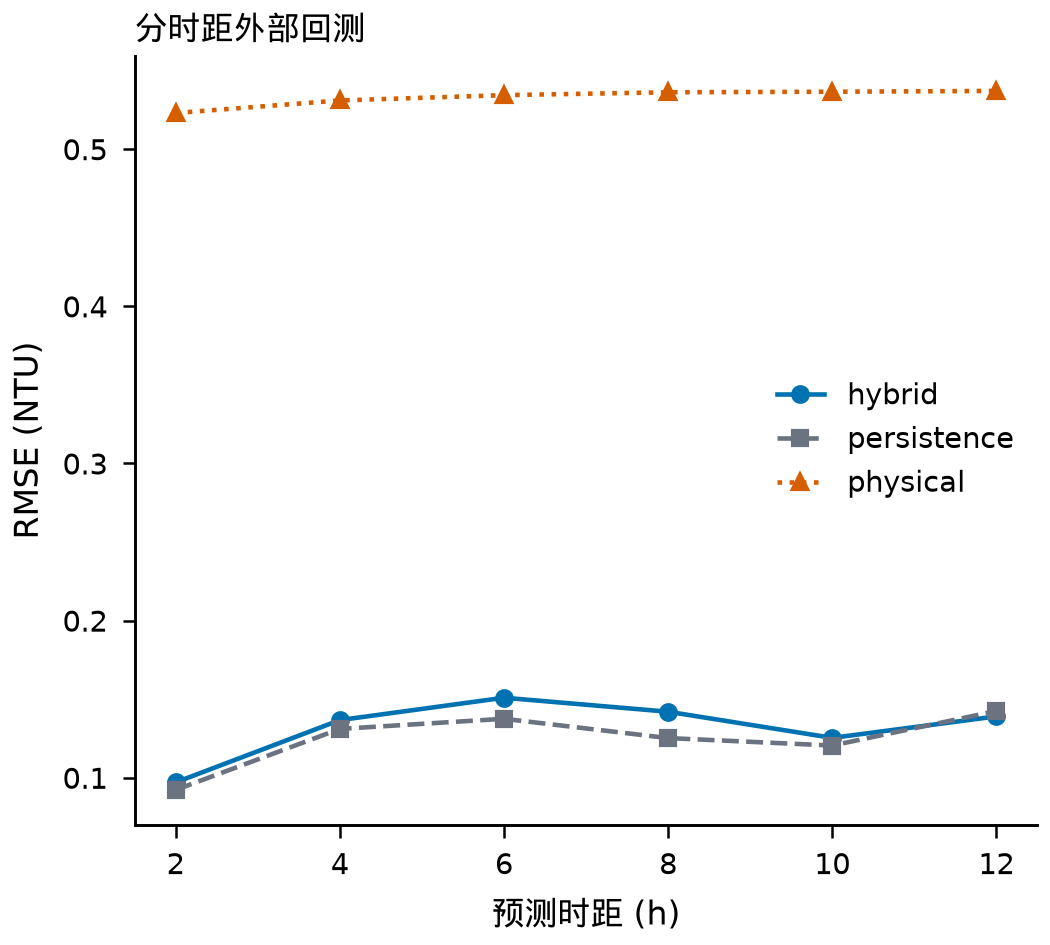
\includegraphics[width=0.53\textwidth]{result_q3_horizon_accuracy.png}
\caption{混合模型、持续性和纯物理基线的分时距 RMSE}
\label{fig:q3-accuracy}
\end{figure}

题目要求 1--12 h 结果，而原始数据分辨率为 2 h。对偶数小时使用独立训练的直接模型；对奇数小时，只在相邻偶数小时轨迹的 $\log(1+Y)$ 尺度做中点插值，并在结果表中设置插值标记。该操作提供时距对齐，不构成新的独立预测模型。情景敏感性显示，在三个指定日 12 h 时，原水浊度增加 100\% 对中心预测的影响约为 0.0064--0.0070 NTU；混凝剂 $\pm10\%$ 的变化多在 $10^{-3}$ NTU 内且方向随时距变化，因此不据此下因果投药建议。

具体地，若 $h$ 为奇数且两侧偶数时距为 $h_-$ 与 $h_+$，则对每条路径定义
\begin{equation}
\log(1+Y_{t+h}^{(b)})=
\frac{1}{2}\left[\log(1+Y_{t+h_-}^{(b)})+\log(1+Y_{t+h_+}^{(b)})\right].
\label{eq:odd-interpolation}
\end{equation}
这种几何尺度插值保持正值，并比 NTU 尺度算术插值更符合前述对数误差结构。由于源数据在奇数小时没有真值，无法计算独立 RMSE 或覆盖率；因此结果表中的插值标记是解释 1、3、5、7、9、11 h 输出时不可省略的证据边界。

情景分析也只改变指定输入并保持其他历史和模型参数不变，回答的是局部条件敏感性而非干预效应。以 2 月 1 日起点为例，原水浊度增加 100\% 时，12 h 中心值由 0.322272 变为 0.329068 NTU，差约 0.006796 NTU；同日起点混凝剂减少 10\% 时，12 h 差约 $-0.000771$ NTU。变化相对预测区间很小，且混凝剂方向随时距改变。这表明现有模型和观测数据不足以支持精细投药优化，合理用途是检验预测对输入扰动是否异常敏感。

\section{问题四：营运日风险评估}

\subsection{幅度、时长与负荷指标}

设营运日 $d$ 的 12 个出厂水浊度为 $Y_{d,r}$，以 1 NTU 为基准定义超额
\begin{equation}
e_{d,r}=\max(Y_{d,r}-1,0),\quad
A_d=\max_re_{d,r},\quad
D_d=2\max\operatorname{run}(e_{d,r}>0),\quad
L_d=2\sum_re_{d,r}.
\label{eq:risk}
\end{equation}
其中 $A_d$ 为最大超标幅度，$D_d$ 为最长连续超标时长，$L_d$ 为 NTU$\cdot$h 意义下的超标负荷。若有效时点少于 9 个，则不直接评级；二月使用问题三的递推轨迹补充，并另报预测比例和等级区间。

三个指标从不同角度描述同一天。$A_d$ 对单次高峰敏感，能够识别持续时间很短但幅度大的事件；$D_d$ 忽略幅度细节，强调超标是否连续；$L_d$ 同时累积幅度与持续时间，可区分两个最大值相同但整体负荷不同的营运日。2 h 系数来自采样间隔，因此 $D_d$ 只能取 0、2、4 h 等离散值，$L_d$ 是矩形求和近似而非连续积分的精确值。当前分级规则直接使用 $A_d$ 与 $D_d$，同时输出 $L_d$ 供解释和后续规则升级。

设四个等级按 $0,1,2,3$ 编码，对第 $b$ 条路径得到 $G_d^{(b)}$，则二月的等级概率为
\begin{equation}
\widehat p_{d,g}=\frac{1}{500}\sum_{b=1}^{500}
\mathbf 1\{G_d^{(b)}=g\},\qquad g=0,1,2,3.
\label{eq:grade-probability}
\end{equation}
众数等级取概率最大的 $g$，区间则取 500 个有序等级的 2.5\% 和 97.5\% 分位位置。由于分级函数包含最大值、连续段和逻辑阈值，通常有“中心轨迹的等级”不等于“路径等级的众数”，也不能把各时点上界拼成一条物理轨迹再评级。逐路径计算保证同一天 12 个时点来自同一个联合样本。

分级规则为：$A_d=0$ 时 SAFE；$A_d\le0.5$ 且 $D_d\le4$ h 时 LOW；$A_d\le1.0$ 且 $D_d\le8$ h 时 MEDIUM；其他为 HIGH。该阈值是为了把幅度和持续时间联合编码的决策设计，不是题目之外虚构的法规条款。图~\ref{fig:q4-maximum} 给出每日最大值和 1 NTU 基准，图~\ref{fig:q4-matrix} 展示各日落在分级矩阵中的位置。

分级采用逐级包含的矩形边界。恰好等于 1 NTU 时超额为零并归 SAFE；最大超额不超过 0.5 NTU 且连续时长不超过 4 h 才可归 LOW，只要任一条件越界就进入更高等级判断。类似地，MEDIUM 要同时满足幅度不超过 1.0 NTU、时长不超过 8 h。逻辑中的“且”防止以很短时长掩盖过大峰值，也防止以很小幅度掩盖长时间连续超标。HIGH 是剩余集合，既包括大幅尖峰，也包括超过 8 h 的持续事件。

\begin{figure}[htbp]
\centering
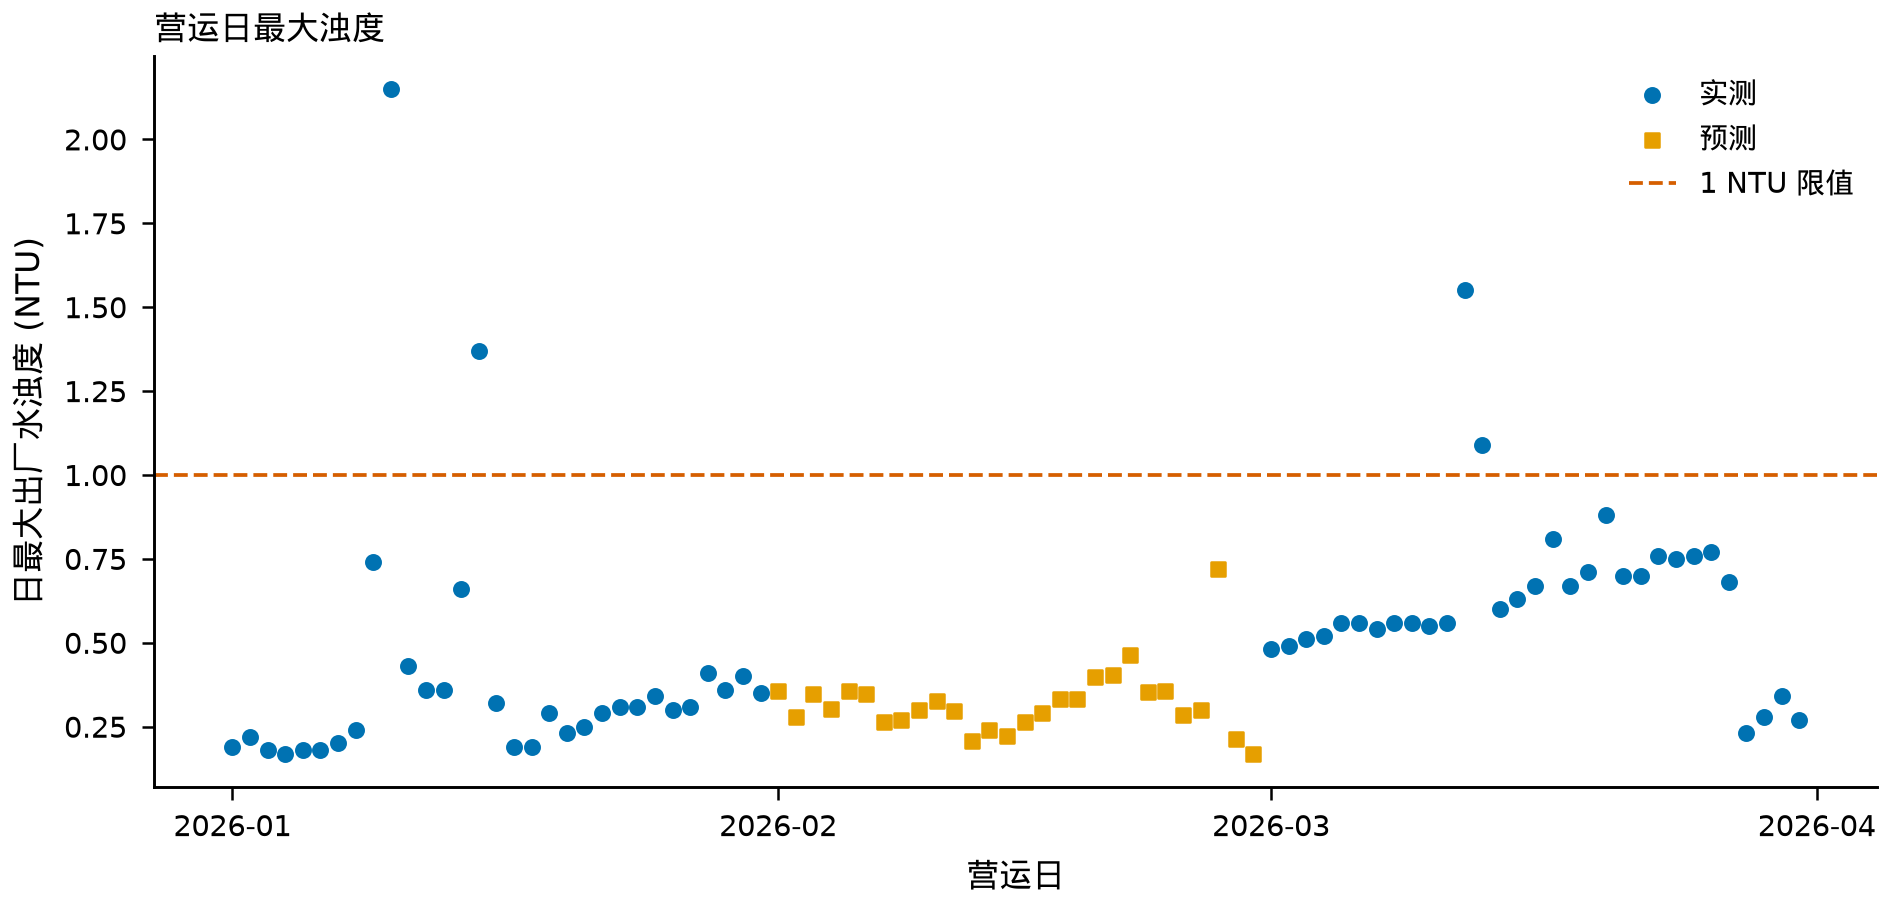
\includegraphics[width=0.88\textwidth]{raw_q4_daily_maximum.png}
\caption{90 个营运日的最大出厂水浊度}
\label{fig:q4-maximum}
\end{figure}

\begin{figure}[htbp]
\centering
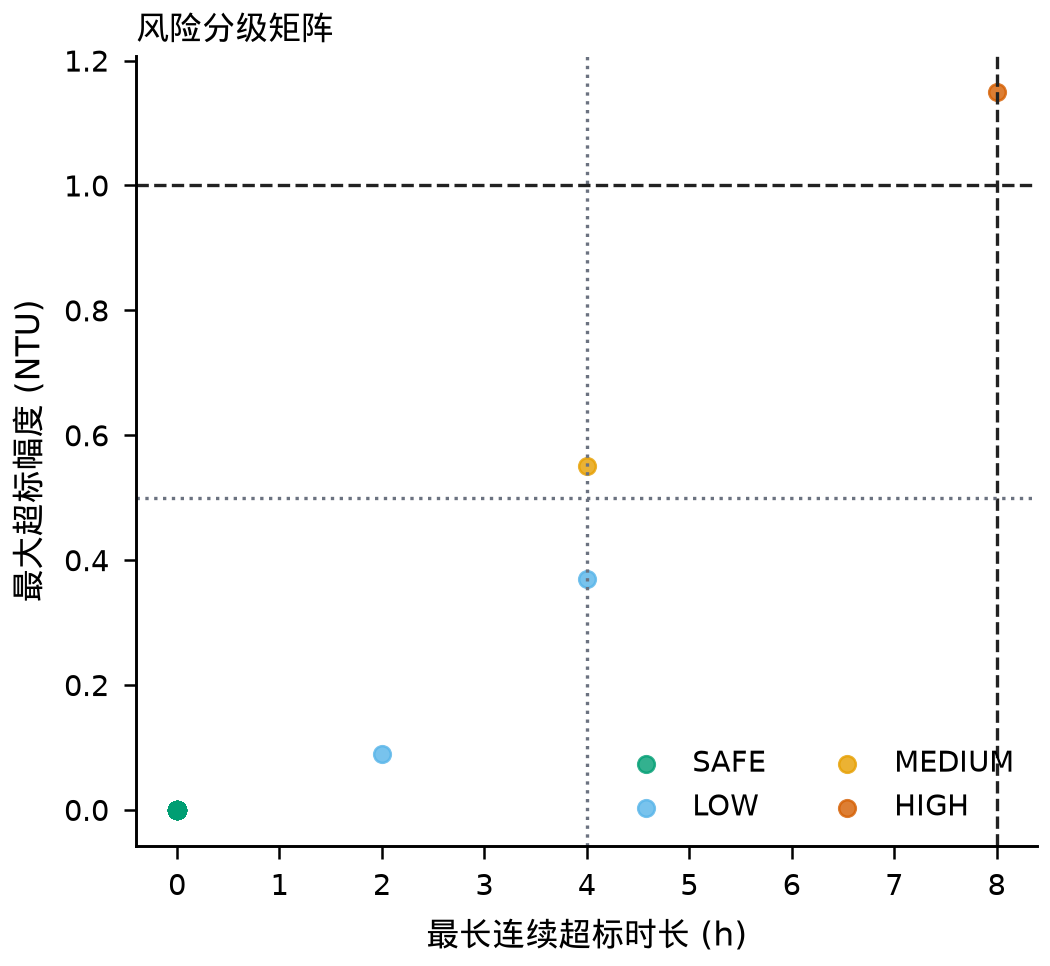
\includegraphics[width=0.53\textwidth]{process_q4_risk_matrix.png}
\caption{最大超标幅度与最长连续超标时长构成的风险矩阵}
\label{fig:q4-matrix}
\end{figure}

\subsection{等级结果与预测不确定性}

90 个营运日的众数等级分布见表~\ref{tab:q4}。3 月 12 日实测最大浊度 1.55 NTU、最大超额 0.55 NTU、最长连续超标 4 h，判为 MEDIUM；3 月 13 日最大浊度 1.09 NTU、连续超标 2 h，判为 LOW。其余 3 月日均为 SAFE。

3 月 12 日是理解二维规则的代表：0.55 NTU 的最大超额已经超过 LOW 的 0.5 NTU 幅度边界，即使连续时长仅 4 h，也不能归 LOW；它同时满足 MEDIUM 的两项上限，故为 MEDIUM。3 月 13 日最大超额仅 0.09 NTU、连续 2 h，落入 LOW。HIGH 日不应只按日最大值解释，还需联合查看连续时长和负荷。表中 86 个 SAFE 是众数统计，其中二月使用预测路径，因此与一月、三月完全由实测形成的 SAFE 在证据强度上不同。

\begin{table}[htbp]
\centering
\caption{2026 年 1--3 月营运日等级分布}
\label{tab:q4}
\begin{tabular}{lrr}
\toprule
等级 & 天数 & 占比/\%\\
\midrule
SAFE & 86 & 95.56\\
LOW & 2 & 2.22\\
MEDIUM & 1 & 1.11\\
HIGH & 1 & 1.11\\
\bottomrule
\end{tabular}
\end{table}

对每条二月轨迹独立评级，再由 500 个等级得到概率、众数和 2.5\%--97.5\% 等级范围。图~\ref{fig:q4-grades} 中竖线表示该范围。二月的中心轨迹均为 SAFE，但 28 天的等级上界没有一天停留在 SAFE：其中 6 天上界为 MEDIUM，22 天为 HIGH。这一结果与问题一的宽区间一致，说明“中心值低于 1 NTU”不能推出缺失月确定安全。

等级区间较宽并不意味着二月实际发生了 22 个 HIGH 日，而是表示在历史误差块支持的联合轨迹中，这些日的高分位等级可以达到 HIGH。相反，众数为 SAFE 也不表示 HIGH 概率为零。中心值回答最典型轨迹的位置，等级上界回答尾部风险可能到达的类别；在缺失期二者必须并列呈现。若营运决策对漏报高风险的代价远大于误报，则可关注 $P(G_d\ge \mathrm{MEDIUM})$；若用于常态资源安排，则还应结合众数、负荷中位数和最新在线观测，不宜只用最坏分位数。

问题一与问题三对二月不确定性的用途不同。问题一给出三个指定营运日、12 个时次的条件预测，适合检查特定日内变化；问题三生成整月连续路径，适合计算连续超标和等级。两者模型结构、残差来源和目标不同，不能把问题一的逐点上下界直接替换问题三路径。二者共同得到“中心偏低但上界宽”的结论，增强了对不确定性方向的定性支持，却仍不能代替二月实测。

\begin{figure}[htbp]
\centering
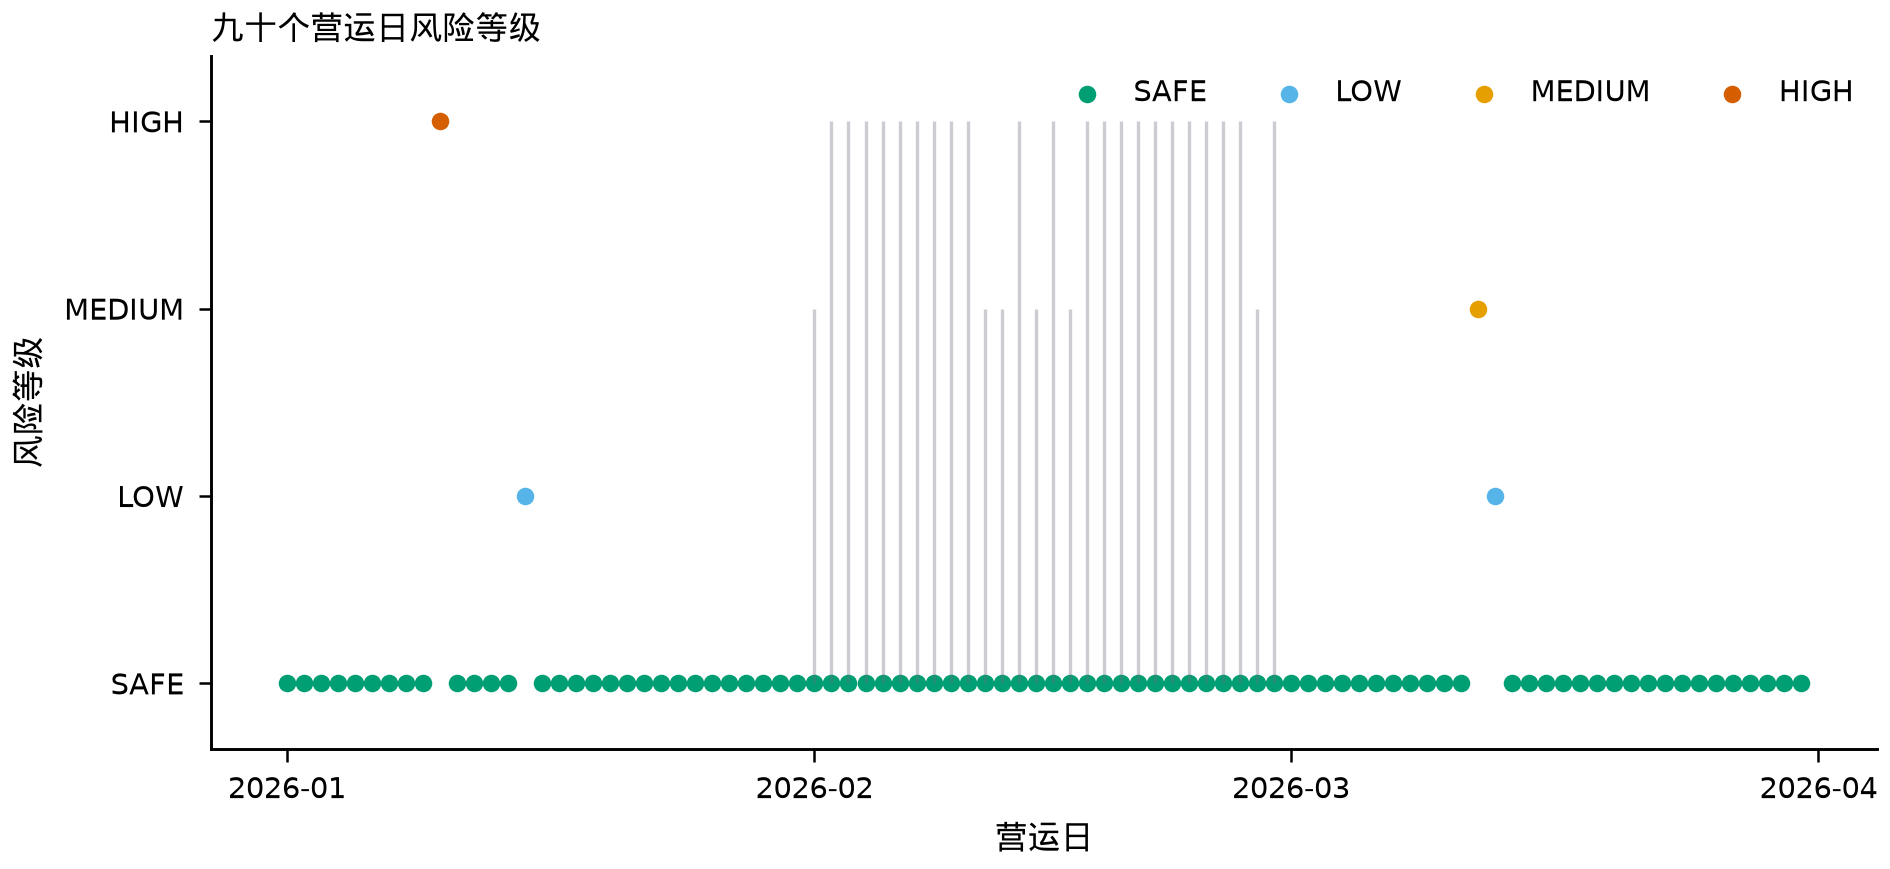
\includegraphics[width=0.88\textwidth]{result_q4_daily_grades.png}
\caption{90 个营运日的众数等级与 95\% 等级范围}
\label{fig:q4-grades}
\end{figure}

\subsection{阈值稳健性}

为检查人为阈值的影响，将 LOW 幅度阈值在 0.4、0.5、0.6 NTU 间变化，MEDIUM 幅度阈值在 0.8、1.0、1.2 NTU 间变化；LOW 时长取 2、4、6 h，MEDIUM 时长取 6、8、10 h，共计算 81 组方案。逐日不变率的均值与最小值均由程序输出。该分析用于说明等级对边界选择的敏感性，而不是从数据中反向挑选能产生更多 SAFE 日的阈值。

81 组方案下，逐日等级相对基准规则的不变率均值为 0.991358，最小值为 0.977778，即最敏感的方案也只有 2 个营运日改变等级。高不变率主要因为绝大多数日的最大浊度离 1 NTU 基准较远，而非阈值设计已经得到法规验证。真正需要人工复核的是靠近分界的少数日期：它们对幅度或连续时长阈值的小调整敏感，且预测日还叠加模型区间。因而稳健性结论应表述为“现有 90 天总体等级分布对这组有限扰动稳定”，不能外推到其他年份、其他水厂或完全不同的风险偏好。

\section{模型评价、适用边界与改进}

\subsection{模型优点}

第一，时间轴按营运日而非自然日构造，并对源文件、语义内容和输出工作簿同时记录哈希，使数据清洗和复现可追踪。第二，问题一采用同一前置训练模型计算基准与置换误差，并把方向一致性落实到四个滚动折，避免因训练窗口混用而改变因素集合。第三，问题三不是纯黑箱外推，而是将质量守恒的 RTD 传播与数据残差修正分离；500 条联合轨迹继续传递到问题四，使等级区间与预测不确定性保持一致。第四，模型选择和结论均保留 3 月外部检验，负 $\Rtwo$、残差相关和基线优胜没有被删除。

\subsection{局限与失败条件}

最主要限制是二月出厂水目标完全缺失，无法在该月校准模型漂移或检验区间覆盖。Q1 的两个模型都在 3 月明显弱于简单前一日基线，表明跨月关系可能发生结构变化。Q2 虽能描述常态水平，但滤后水尖峰稀少且难预测，残差诊断未通过白噪声门槛。Q3 的物理基线采用单参数指数 RTD，无法表示旁路、分层或多池串联；混合模型在短中时距也未稳定超过持续性。风险分级阈值是解释性设计，只有在水厂或监管方确认后才能作为正式操作规则。

模型还假设各输入的源表含义跨月份一致。原水 pH、出厂 pH、余氯和混凝剂等变量约有 30\% 缺失，虽然训练内中位数填补避免删除大量样本，但会削弱它们的可识别贡献。变量之间还受操作控制闭环影响，例如高色度可能触发投药调整，因此条件效应只代表现有运行策略下的统计关联。

\subsection{改进方向}

后续应首先补齐二月化验或在线传感器记录，并增加跨年度外部月份；其次记录反冲洗、设备切换、降雨和投药设定点变化，为尖峰建立事件标签；再次通过示踪试验或池体几何取得 RTD 参数，可将单指数核扩展为多槽串联或旁路模型。统计层面可采用随时间变化的状态空间系数、尖峰和常态的两阶段模型，以及带在线校准的概率预测。上述改进的评价标准仍应以外部月份、持续性基线和区间校准为核心，而非只比较训练误差。

\section{模型链路核验与营运使用}

\subsection{四问接口与误差传递}

表~\ref{tab:modelchain} 将四问的输入、输出、验证证据和停止条件并列。该表的作用不是重复结果，而是说明哪些量可以跨问题传递。Q1 和 Q3 都涉及出厂水预测，但职责不同：Q1 以全部同期条件变量解释指定日，Q3 从滤后水传播和历史残差生成连续路径。Q2 的输出是滤后水动态关系及有效时滞，不直接作为 Q3 的未来滤后水预测器；Q3 使用已经观测或情景给定的上游信息。Q4 只接收 Q3 的联合路径或完整实测日，不接收互相独立的逐点上下界。

\begin{table}[htbp]
\centering
\caption{四问模型接口、验证证据与使用限制}
\label{tab:modelchain}
\begin{tabular}{L{0.7cm}L{3.0cm}L{3.3cm}L{3.5cm}L{3.0cm}}
\toprule
问题 & 主要输入 & 输出 & 外部或稳健性证据 & 停止或降级条件\\
\midrule
Q1 & 过程变量当前与滞后项 & 因素、条件预测区间 & 三月模型弱于前一日基线 & 不宣称跨月泛化\\
Q2 & 四项外生输入及滤后历史 & 有效时滞、滤后条件均值 & 三月负 $\Rtwo$、残差相关 & 不作尖峰保证或因果控制\\
Q3 & 滤后水、RTD 与出厂残差状态 & 1--12 h 联合预测轨迹 & 六时距回测及持续性比较 & 短中时距优先保留基线\\
Q4 & 完整实测日或 500 条路径 & 日指标、等级概率与范围 & 81 组阈值扰动 & 预测日不得只报众数\\
\bottomrule
\end{tabular}
\end{table}

误差沿链路传播时应区分参数不确定性、残差不确定性和结构不确定性。500 条路径主要表达历史多时距残差在当前模型下的随机变化，尚未完整覆盖“RTD 形式选错”“回归系数跨月漂移”等结构风险。Q1 在三月的失败恰好证明结构偏移可能大于常规残差。因此，Q4 的等级上界虽然比单一中心值更审慎，也不能被解释为包含所有可能风险的绝对保证。若新时期的残差分布或输入范围明显越出训练期，应暂停概率解释并触发重新校准。

四问的负面检验结果还决定了模型组合方式。Q1 中非线性 RFF 虽优于 Huber 岭，却仍远弱于前一日基线，说明仅增加非线性复杂度不能解决跨月漂移；Q2 增加 AR 阶数也未消除相关残差；Q3 仅在 12 h 略优于持续性。因而最终系统不采用“始终选择复杂模型”的固定规则，而应把基线作为常驻候选：2--10 h 在线点预测可并列显示持续性与混合模型，二者分歧超过历史误差尺度时标记为模型不一致；12 h 可采用混合中心，但仍显示持续性参照。这个策略将失败证据转化为使用规则，而不是只写在局限章节。

\subsection{营运研判流程}

建议把一次在线研判划分为数据门、预测门和风险门。数据门首先检查时间轴是否仍为 2 h 间隔、关键输入是否可解析、最近 12 h 的滤后与出厂历史是否齐全；若某营运日有效点少于 9 个，则实测日不直接评级。还要检查新输入是否超出训练期 0.5\%--99.5\% 范围。缩尾能使程序继续运行，却不能证明极端工况仍处于模型适用域，因此应同时保留越界标记供人工查看。

预测门在数据通过后计算两套参照。对指定日期的条件补充，输出 Q1 中心、95\% 区间和前一营运日同次基线；若复杂模型持续弱于基线或区间显著扩张，界面应突出“不具跨月泛化证据”。对 1--12 h 预报，偶数时距输出混合、持续性和区间，奇数时距明确标识为插值。若发生滤后水尖峰、反冲洗或设备切换而历史中缺少同类事件，应将预测标为事件外推，不据中心曲线安排自动控制。

风险门按路径而非点区间计算 $A_d,D_d,L_d$。实测完整日直接给出确定等级；二月式缺失日同时给出众数、各等级概率和 95\% 等级范围。若众数为 SAFE 但上界达到 MEDIUM 或 HIGH，应进入人工复核队列，核对在线仪表、原水变化和运行日志；不能用 SAFE 众数关闭告警。若实测或路径中出现 HIGH，首先回看构成 HIGH 的原因是幅度、连续时长还是二者共同越界，因为三种情形对应的现场排查重点并不相同。

上述流程不直接给出投药量建议。Q3 情景分析中，混凝剂变化的预测差仅在 $10^{-3}$ NTU 量级且方向不稳定，Q1 的原水色度负效应也明显受控制闭环影响。在缺少随机试验、可靠过程机理或可识别工具变量时，回归条件效应不能支持自动干预。模型更适合做数据完整性检查、短期趋势参照、异常日排序和人工研判的信息汇总层。

\subsection{更新、监控与失效判据}

部署后应按营运日保存预测时刻、可用输入、模型版本、基线、中心区间和最终实测。每月重新计算各时距 RMSE、MAE、$\Rtwo$、95\% 覆盖率以及模型相对基线的误差差
\begin{equation}
\delta_h=\mathrm{RMSE}_{\mathrm{model},h}-
\mathrm{RMSE}_{\mathrm{baseline},h}.
\label{eq:monitor}
\end{equation}
当 $\delta_h>0$ 时，表示该时距没有增量优势；连续多个评估窗为正时应降级到基线并重训，而不是继续沿用旧模型。覆盖率显著低于名义水平表示区间过窄，显著高于名义水平且区间很宽则表示虽少漏报但信息价值不足，两者都需要重新校准。

残差监控不能只看均值。Q2 已出现最大绝对 ACF 0.416470，故更新时需继续计算 Ljung--Box 检验和分滞后 ACF；若相关性增强，移动块长度也应重新选择。对输入分布可监测中位数、四分位距、缺失率和越界率；对输出则单独统计常态段与尖峰段误差，避免大量低值掩盖少数关键事件。新收集到反冲洗、切换或降雨标签后，可将尖峰预测拆为“事件发生概率 + 事件幅度”的两阶段问题。

模型重训必须保留旧版外部测试结果，不能用加入三月后的全量训练拟合来覆盖原先失败证据。合理流程是随时间前推：例如加入三月后，用更晚月份作为新的未见测试窗，并继续与相同营运时次前一日和持续性比较。只有多个独立月份都显示稳定增益，才可提高模型的使用等级。若二月实测被补回，应首先作为锁定测试集评估原始二月预测，而不是先参与重训；否则将失去检验本次缺失期推断是否可靠的唯一机会。

\subsection{可复现性与证据绑定}

复现链从只读输入开始。15 个源工作簿分别记录字节哈希和解析后的语义哈希，前者检测文件任意变化，后者检测影响记录内容的变化。程序固定随机种子并重建 5460 行时间轴、全部 CSV、500 路径数组、12 幅正式图与结果工作簿。工作簿含 346 个公式，经 LibreOffice 重算后检查公式错误为 0；复现清单同时绑定代码、数值汇总、工作簿字节哈希和语义哈希。这些证据使“源表未改、代码实际运行、工作簿公式已重算”成为可分别核验的事实。

论文层以单一 \LaTeX{} 主稿为来源，Word 由该主稿转换，避免两个版本分别手工维护后出现数值分叉。图表只引用复现目录中的冻结结果，正文精度统一从 CSV 或 JSON 取得。构建清单记录主稿哈希、编译后主稿哈希和 PDF 哈希；三者相互绑定时，能够证明交付 PDF 对应当前源稿。引用的 8 篇文献均通过两个论文数据源交叉匹配，并进一步核对 DOI、出版社或 PMLR 元数据；文献只用于支撑方法背景，不替代本数据上的实证结果。

可复现不等于结论必然正确。哈希能证明输入和输出未被悄然替换，固定种子能证明随机过程可重复，严格编译能证明版面没有已知警告；它们不能消除模型结构偏差或缺失月不可验证的问题。因此交付中同时保留负 $\Rtwo$、基线比较、残差相关和等级宽区间。完整证据链的价值正是让读者能够重现成功结果，也能够重现模型失败与适用边界。

\section{结论与复现说明}

本文完成了从原始表格到营运风险的闭环建模。稳健筛选得到滤后水浊度和原水色度两项主要关联因素，但问题一跨月泛化失败；问题二给出 2、0、0、6 h 的有效输入时滞，同时暴露明显残差相关；问题三得到 8 h 的 RTD 时间尺度和 500 条联合轨迹，但混合预测仅在 12 h 略优于持续性；问题四显示 90 天中 86 天众数等级为 SAFE，同时揭示二月等级范围的显著不确定性。因此最稳妥的使用方式是把模型作为缺失期辅助研判和异常筛查工具，并始终并列展示基线、区间和外部检验，不用中心预测替代实际监测。

全部结果由固定种子 20260727 产生。唯一编程复现命令为 \texttt{PYTHONPATH=.vendor python reproduce.py}；它重建数值结果、12 幅彩色及灰度审查图、结果工作簿、LibreOffice 重算证据与哈希清单。输入文件保持只读，问题三轨迹数组维度为 $500\times5460$。论文中的表格数值均取自同一结果目录，未人工重算或替换。

复现完成后应按“数据行数与时间轴、四问核心数值、工作簿公式错误、图表契约、文件哈希”的顺序核对。只有 5460 个时点、336 个二月目标缺失、四问指标和 500 条路径均与清单一致，且工作簿重算无错误时，才把本次运行视为同一证据版本；任一环节变化都应生成新的清单并重新构建论文，而不能只替换最终 PDF。

\bibliographystyle{plain}
\bibliography{references}
\end{document}
